\documentclass{article}

\usepackage{authblk}
\usepackage{geometry}
\usepackage{t1enc}
\usepackage[english]{babel}
\usepackage{csquotes}
\usepackage[sorting=none, backend=biber, style=numeric]{biblatex}
\usepackage{graphicx}
\usepackage{caption}
\usepackage{subcaption}

\graphicspath{ {Pictures/} }
\addbibresource{Bibliography/RouteProfileRecording.bib}

\renewcommand\Affilfont{\small}

\geometry{
	a4paper,
	margin=1in}

\title{Methods for recording railway route profiles for vehicle dynamic simulation}

\author{Tamás DEMUS}
\author{Máté M. SZŰCS}
\author{István ZOBORY}
\affil{Department of Railway Vehicles and Vehicle System Analysis\\
Faculty of Transportation Engineering and Vehicle Engineering\\
Budapest University of Technology and Economics\\
H-1111 Budapest, Műegyetem rkp. 3, Hungary}

\date{\today}

\begin{document}
	\pagenumbering{gobble}
	\begin{titlepage}
		\maketitle
		\begin{abstract}
			Railway vehicle dynamics simulation can be performed in several ways. A key factor on the output of such simulation is the parameter set used. Track and vehicle information can be gathered from operators, but control functions are not available in all cases. Identification of these traction and brake control functions is essential. Current research focuses on defining the tools to gather data from real life measurements on order to obtain the desired information. In this paper a series of measurement is conducted under different conditions and with different tools to identify the best device for later research purposes. Focus is put on self-developed tools equipped with different GNSS receivers. Static and dynamic measurements and a field test is carried out and the obtained data is analyzed to compare the performance of the devices used: an iPhone 11 Pro mobile phone and two GNSS receivers applied on the ARDUINO platform. The analysis focuses on the reliability and the achived accuracy of the tools in terms of location, altitude and speed information. A proposal is made which tool to use for extended measurements in the future. The gathered information can be used at a later step of the research to determine track parameters, investigate the realizations and compare with the planned route. \\
			\\
			Keywords: GNSS, railway track, railway vehicle, train positioning, route profile, vehicle dynamics, arduino
		\end{abstract}
	\end{titlepage}	
	\pagenumbering{arabic}
	\section{Introduction}
		Simulating rail vehicle dynamics require reliable input data in terms of track and vehicle parameters and control functions for traction and braking. Obtaining proper control functions difficult as it depends on many factors, such as track condition, vehicle traction mode, driving style, traffic situation or unexpected events. Current research focuses on measurement tools developed to record train route profiles which serves as a basis for determining control functions for later simulations. \\
		The developed tools rely on GNSS technology that is widely used for positioning purposes and subject of extended research in the railway industry. A brief summary about the general application of GNSS technology can be found in \cite{GNSSApplicationsWikipedia}, \cite{GNSSApplicationsNavipedia} while railway applications listed in \cite{RailApplicationsNavipedia} and \cite{salmiInventionsUtilizingSatellite2009}. Current section gives a short overview about the application of GNSS technology for railway track measurements and train positioning and introduces handheld devices developed for solving positioning problems.\\
		Railway track measurement utilizes a range of methods to determine the exact geometry of the track including the position, elevation, curvature, cant, relative position of the rails and so on \cite{MeasuringTestingEquipment}. Common in these methods is that they require measurements done manually and often considered to be a very slow process. To avoid the issue of lengthy measurements GNSS technology is being used to record track geometry. To determine whether the required accuracy can be achieved, extended research program is being carried out at the Gda\'{n}sk University of Technology and the Maritime University of Gdynia as part of the InnoSatTrack project \cite{InnoSatTrackFacultyElectrical}. Several configurations of GNSS receivers studied, results show that accuracy level of 3 mm to 6 mm can be achieved during inventory of railway tracks that allows the study of track deformation \cite{spechtAnalysisTramTracks2017}. It is also indicated that the speed of the receiver during measurement influences the accuracy due to the dynamics of the vehicle, therefore sampling and filtering should be set in a way to allow statistical tools to be used \cite{spechtVerificationGnssMeasurements2020}. For such measurement an increase in accuracy is observed when using multi-mode GNSS receivers \cite{spechtTestingPositioningAccuracy2020}. The research carried out in these projects utilized high-end GNSS receivers with RTK mode and corrections via the GPRS network to mitigate the effect of obstacles around the rail track.\\
		GNSS technology is widely used in not safety critical applications for train positioning. Extended research is in progress to study the application for safety critical applications under the Shift2Rail program \cite{HomeShift2Rail}. An overview of positioning research is given in \cite{oteguiSurveyTrainPositioning2017} and in \cite{spinsanteHybridizedGNSSApproachesTrain2020}. Field research of different technologies and proposal for processing the recorded data is described in \cite{oteguiEvaluationExperimentalGNSS2019}. A specific overview is given in \cite{maraisSurveyGNSSBasedResearch2017} with focus to railway signalling applications. Common in the approach is that GNSS receivers are supported by additional sensors to improve dead reckoning features of the system to avoid signal or accuracy losses. \\
		Several applications of the GNSS technology can be found using low-cost GNSS receivers in combination of small electronic control units, for example the ARDUINO platform \cite{ArduinoHome}. These low-cost solutions can be used for simple tasks, for example positioning and tracking of cars or anti-theft solutions. Some examples can be found in these articles: \cite{costanzoArduinoBasedSystem2013}, \cite{mokhinRealTimeVehicleTracking2018}, \cite{molooLowCostMobileGPS2011}, \cite{moralloVehicleTrackerSystem2021} or \cite{rahmanRealTimeGoogle2016}. Common in these solutions that they utilize a GSM module to transfer the data via the mobile network to the user. Besides these small electronics the opportunity of using the GNSS receivers built-in to mobile phones is also targeted by research work. A comparison of different mobile phones in terms of accuracy can be found in \cite{szotComparativeAnalysisPositioning2019}.\\
		Target of the current study is to develop low-cost solution for recording route profiles of trains. The recorded data later will be used in several different ways:
		\begin{itemize}
			\item Calculate the track parameters of elevation, curvature
			\item Determine maximum allowed speed
			\item Estimate traction and brake force and their control functions
			\item Compare recorded realizations of route profiles with results of numeric simulation and planned profile
			\item Extend measurement scope to different routes to investigate the effect of different parameters of the railway transportation, track and vehicle system
		\end{itemize}
		To achieve these goals the results of the current study has to be evaluated further during later steps in the research. As a first step the following assumptions and considerations have been taken:
		\begin{itemize}
			\item Low-cost and easily available components to be used
			\item No interruption to the railway traffic is possible to obtain real realizations
			\item No GSM connection considered, data is stored in an SD card, therefore augmentation via Internet or GSM network is not possible
			\item No additional sensors are installed to limit complexity and cost level of the system, therefore dead-reckoning is very limited
			\item Different sampling frequencies to be used to evaluate the influence
			\item Processing of data is done off-line
			\item Different protocols can be used for different receivers
		\end{itemize}
	\section{Methodology}
		\subsection{Track and vehicle}
			The line no. 80 and 80a between Budapest-Keleti and Füzesabony stations was selected for the trial measurements (Figure \ref{fig:line_no80}). The line is operated by MÁV-START Co. and part of the Budapest-Keleti to Eger route. It has two standard gauge track with an electrification of 25kV and 50 Hz. The Inter Regio type of train was selected for the measurements which has 10 stops during this section and consits of 2 STADLER FLIRT EMUs coupled together except for the early and late times of the day with an overall of 16 pairs of trains every day. The ride takes 1 hour and 31 minutes, the route is 125 km long and can be divided into three main sections:
			\begin{enumerate}
				\item Budapest-Keleti to Rákoscsaba: lower speed limits, urban area of Budapest, many obstacles around the railway tracks
				\item Rákoscsaba to Hatvan: Gödöllő Hills area, curves with lower radius, wooded area
				\item Hatvan to Füzesabony: plain area, no obstacles, mainly straight sections
			\end{enumerate}
			The section between Rákos and Hatvan is recently renovated and thus giving good track condition. The EMUs are relatively new ones resulting in a good running characteristics offering a good comparison opportunity between the first two sections and the third one.
			\begin{figure}[h]
				\centering
				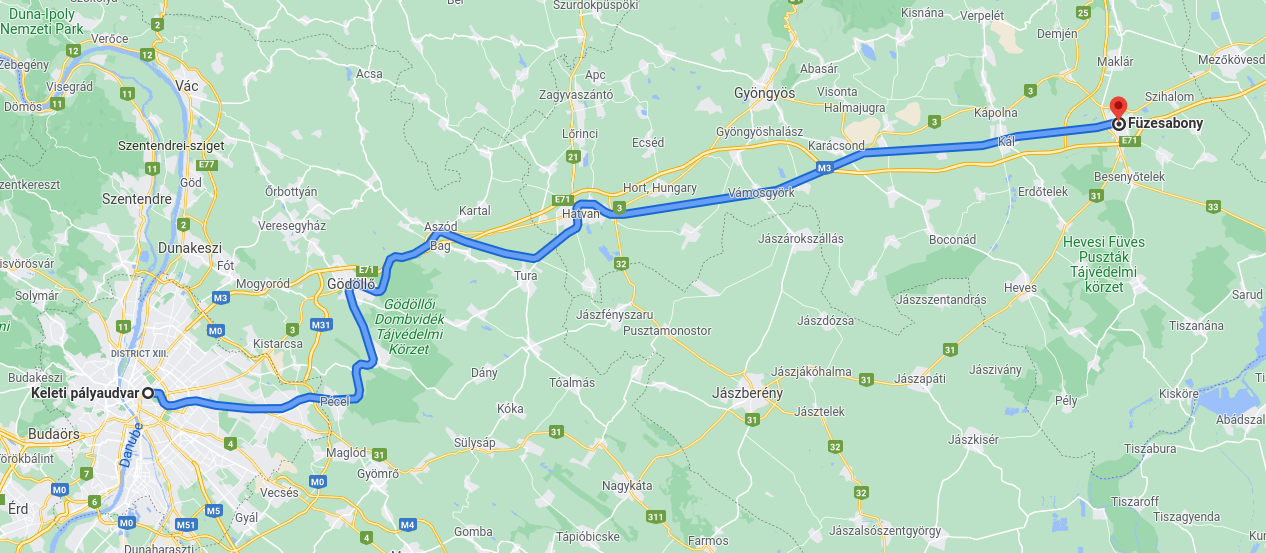
\includegraphics[width=0.9\textwidth]{line_no80.png}
				\caption{Line no. 80 - Budapest-Keleti to Füzesabony}
				\label{fig:line_no80}
			\end{figure}
		\subsection{Measurement devices}
			Three devices were used to carry out the measurements: a mobile phone and two self-made electronics based on the ARDUINO platform equipped with different GNSS receivers. \\
			The mobile phone type is iPhone 11 Pro with iOS 14 operating system. The application Trail Tracker 1.3.4 was used for the measurements. There is no detailed information available on the type of GNSS receiver used, however from the recorded data we can deduct that the sampling frequency is 1 Hz when a satellite fix is found and multi-mode operation is enabled. The app records and stores the data in GPX format \cite{GPXSchemaDocumentation} that is later used for processing off-line. \\
			The first self-made equipment (U-blox M8N) is built from an ARDUINO UNO motherboard and the NEO-M8N receiver made by U-Blox \cite{NEOM8SeriesUblox} and is shown on Figure \ref{fig:gadget1}. An active GNSS antenna is connected to the receiver. The data is recorded to an SD card. The power supply for U-blox M8N is a high-capacity power bank to allow numerous and long test runs. The algorithm for the tool is developed in the ARDUINO IDE environment. It starts by initializing the communication on the serial port, with the receiver and with the SD card. The setup of the GNSS receiver is set to 5 Hz sampling rate and the NMEA messages are disabled. The UBX protocol \cite{UbloxUbloxM82021} is used for the communication between the receiver and motherboard. The UBX-NAV-PVT message is used for transmitting the GNSS information from the receiver that is sent out with a 5 Hz rate. This solution provides general navigation, position, velocity and time information. The messages then parsed by the software and the recorded information is written to the SD card line by line. \\
			The second tool (MTK 3339) is also based on an ARDUINO UNO motherboard but with a combination of an MT 3339 GNSS receiver made by MediaTek Labs \cite{MT3339MediaTekLabs}. The receiver has an active antenna attached. The power supply is solved by the same high-capacity power bank and the data is also recorded to an SD card. In this case the GNSS receiver and the SD card was available in an integrated shield design \cite{OverviewAdafruitUltimate} resulting in a simpler design of the electronics. MTK 3339 is presented on Figure \ref{fig:gadget2}. The software is written in the ARDUINO IDE environment, for the communication the NMEA messages, more precisely the \$GPGGA and \$GPRMC sentences were used which were parsed with 10 Hz sampling rate by the TinyGPSPlus parser \cite{TinyGPSArduiniana} that is freely available. The parsed data was saved to the SD card line-by-line. \\
			For convenient measurements U-blox M8N and MTK 3339 is placed to an aluminium briefcase. The recordings with all tools were done parallel therefore a comparison of the recorded data is possible. Table \ref{table:toolparams} summarizes the main parameters of the tools, the recorded dataset for each solution can be found in Table \ref{table:datasets}. The dataset is different for each tool due to the different software solution applied, this can be unified at a later step of the research. \\
			\begin{figure}[h]
		   		\centering
		     	\begin{subfigure}[b]{0.45\textwidth}
		      		\centering
		      	  	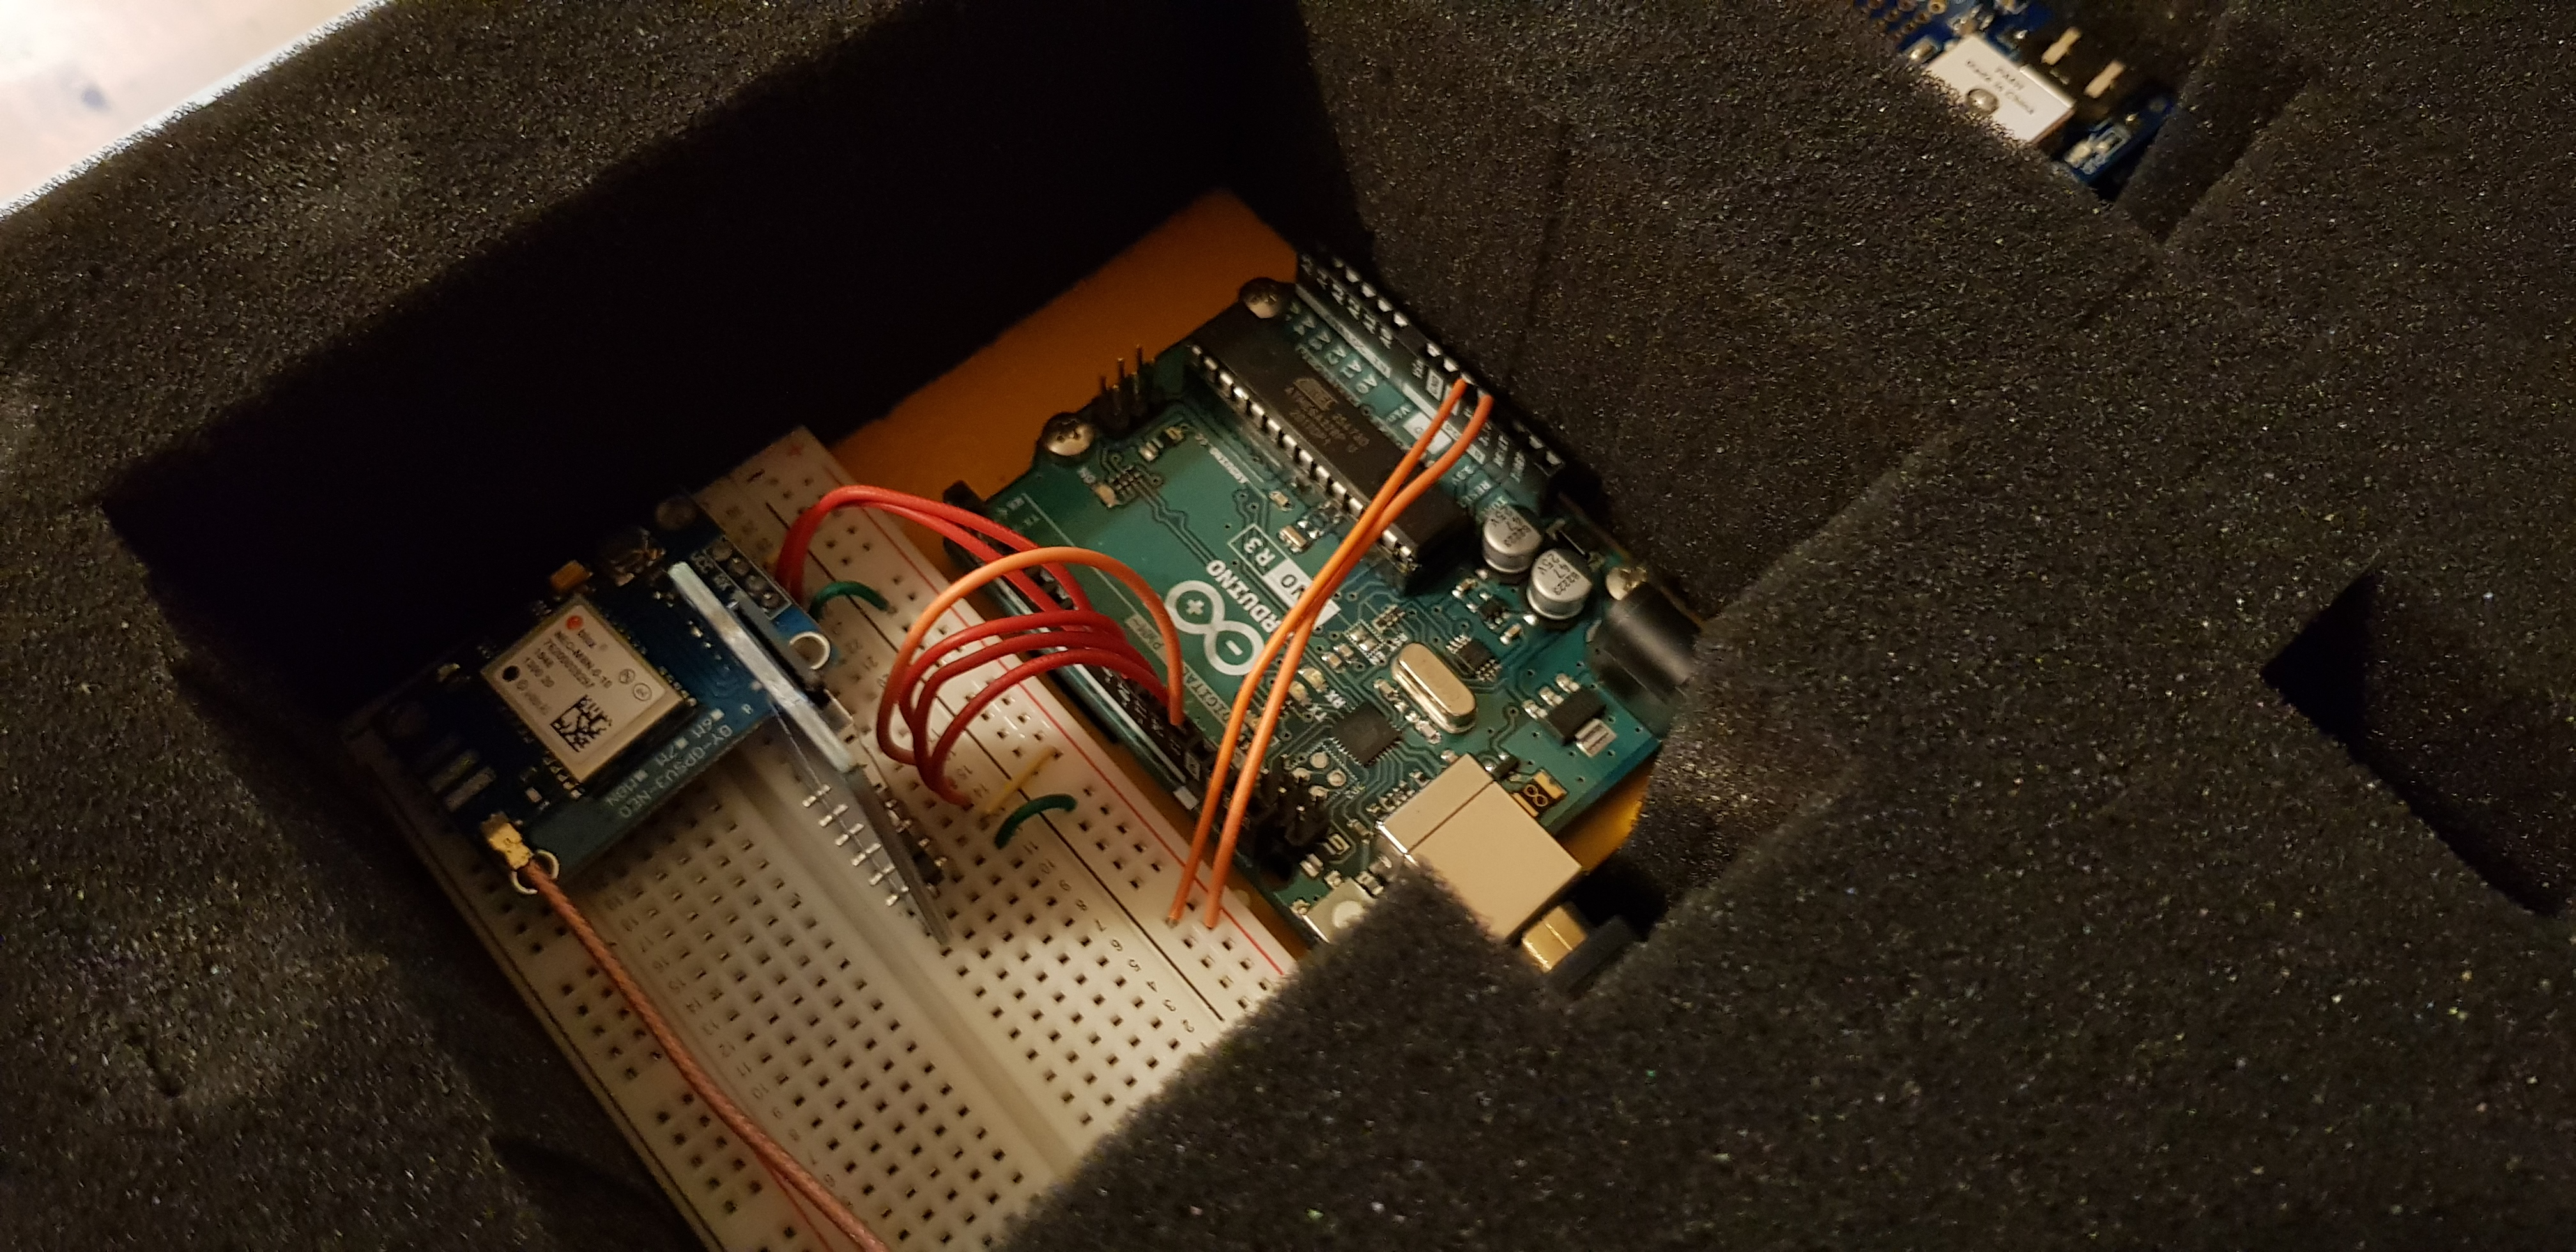
\includegraphics[width=\textwidth]{gadget_1.jpg}
		      	   \caption{U-blox M8N}
		      	   \label{fig:gadget1}
		     	\end{subfigure}
		     	\begin{subfigure}[b]{0.45\textwidth}
		      	   \centering
		      	   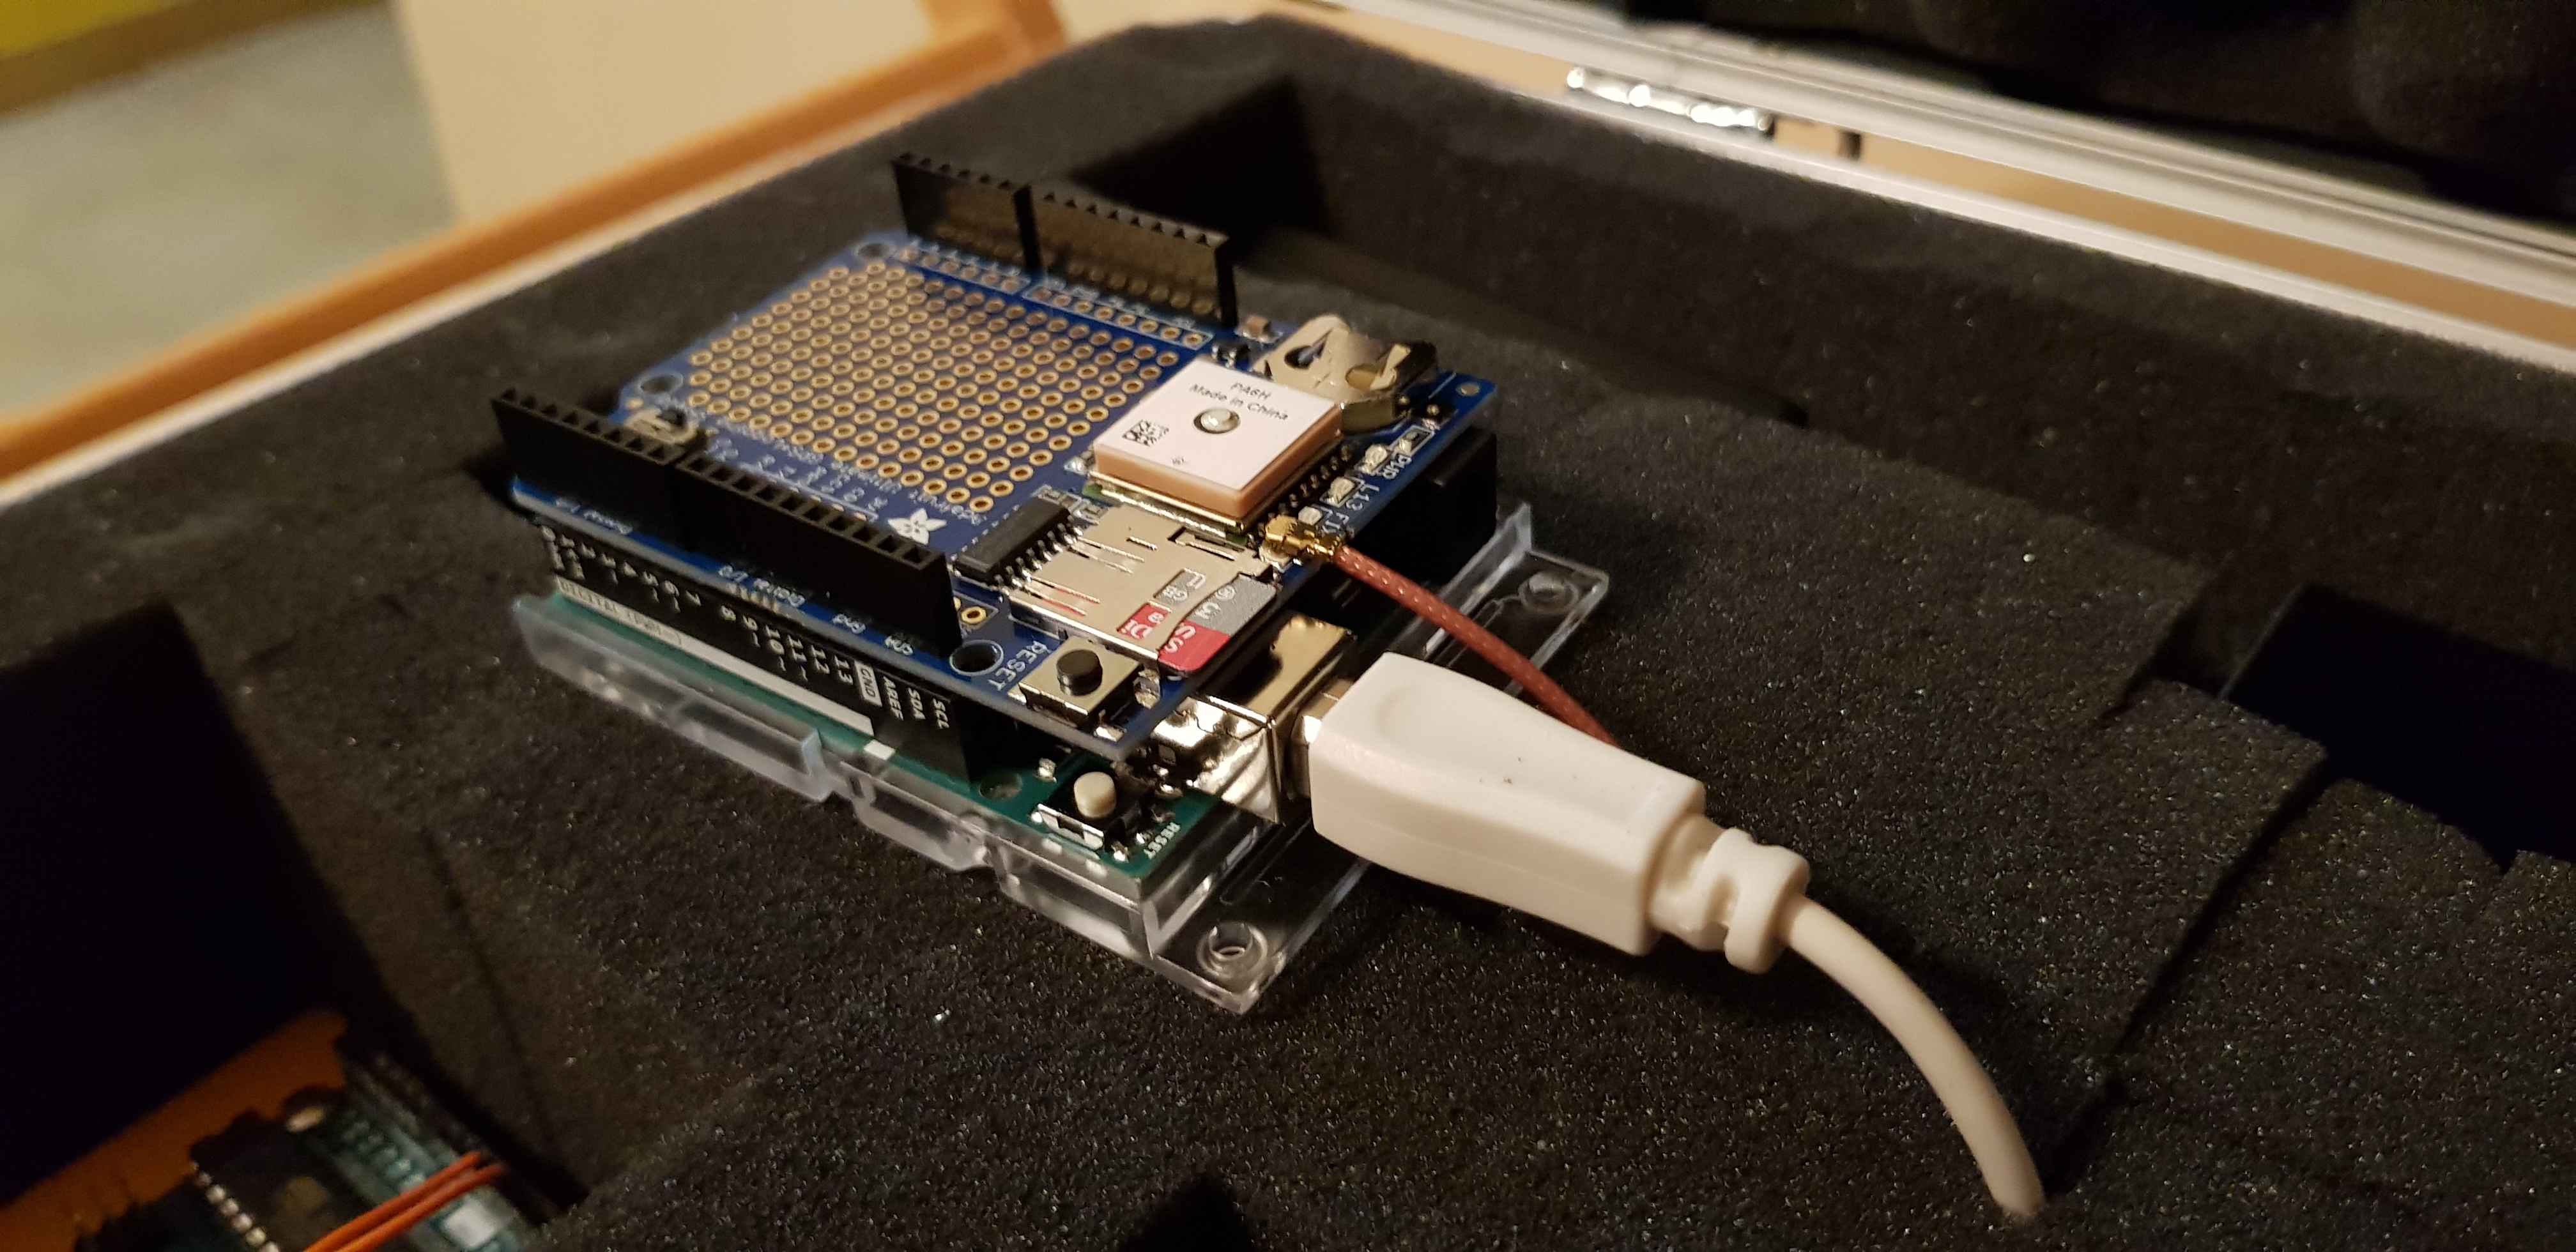
\includegraphics[width=\textwidth]{gadget_2.jpg}
		      	   \caption{MTK 3339}
		      	   \label{fig:gadget2}
		     	\end{subfigure}
		      \caption{Gadgets used for recording route profiles}
		      \label{fig:gadgets}
			\end{figure}		
			\begin{table}[h]
				\centering
				\begin{tabular}{|c|c|c|c|}
					\hline 
					& Mobile phone & U-blox M8N & MTK 3339 \\ 
					\hline 
					Hardware & iPhone 11 Pro & ARDUINO UNO & ARDUINO UNO \\ 
					\hline 
					GNSS receiver type & Built-in & U-Blox NEO-M6N & MediaTek Labs MT 3339 \\ 
					\hline 
					Antenna & internal & active external & active external \\ 
					\hline 
					Operating system & iOS 14 & self-made & self-made \\ 
					\hline 
					Recording software & Trail Tracker 1.3.4 & self-made & self-made \\ 
					\hline 
					Communication messages & not known & UBX-NAV-PVT & \$GPGGA \$GPRMC \\ 
					\hline 
					Parser & built-in & self-made & TinyGPSPlus \\
					\hline 
					Sampling rate & 1 Hz & 5 Hz & 10 Hz \\ 
					\hline 
					File format & GPX & CSV & CSV \\ 
					\hline 
				\end{tabular} 
				\caption{Overview of tool parameters}
				\label{table:toolparams}
			\end{table}
			\begin{table}[h]
				\centering
				\begin{tabular}{|c|c|c|c|}
					\hline 
					& Mobile phone & U-blox M8N & MTK 3339 \\ 
					\hline 
					Longitude & X & X & X \\ 
					\hline 
					Latitude & X & X & X \\ 
					\hline 
					Altitude & X & X & X \\ 
					\hline 
					Date & X & X & X \\ 
					\hline 
					Time & X & X & X \\ 
					\hline 
					Speed & X & X & X \\ 
					\hline 
					Number of satellites & & X & X \\ 
					\hline 
					Horizontal dilution of precision & X & & X \\ 
					\hline 
					Vertical dilution of precision & X & & \\
					\hline 
					Position dilution of precision & & X &  \\ 
					\hline 
				\end{tabular} 
				\caption{Recorded data sets}
				\label{table:datasets}
			\end{table}
		\subsection{Data processing}
			The recorded data is processed further with a script developed in Python programming language. During the post-processing of the data two different status of the processing is distinguished. Raw data refers to the recorded data without any alteration. Conditined data refers to the status after general data cleansing is done. \\
			The data cleaning process aims to find single data points that needs to be excluded from further processing, for example speed information recorded above the maximum allowed speed of the vehicle or corrupted data points. The first step is to identify and drop if any corrupted data is present in the time series of the recordings. \\
			Second step of the conditioning is to remove highly uncertain points from the evaluation therefore the dilution of precision (DOP) information is analyzed and measurement points with DOP value above 20 are removed as these considered to be inaccurate according to \cite{tahsinAnalysisDOPIts2015}. Low number of satellites present for a GNSS fix is removed due to low accuracy. The minimum number of satellites of 7 is selected for the current study. \\
			The remaining time series then analyzed for outliers by calculating the rolling means with a window of 50. The rolling means are used to normalize the recorded values and the standard deviation of the normalized series calculated. The treshold is that each recorded point has to be in \textpm 3 standard deviation range. The calculation is performed for the longitude, latitude, altitude and speed values. Once all the corrupted and outlying points are removed a Savitzky-Golay filter was applied to the series to smooth the dataset as proposed by \cite{wilkDigitalFilteringRailway2020} considering a window of 11 elements and an order of 2. At this point the conditioned dataset is produced. \\
			Increasing the number of points for a later statistical analysis on the stochastic behaviour of the route realizations requires several recordings to be done under similar conditions as far as possible. The resulting realizations needs to be aligned to each other. As no reference point of the measurements given the offset between the different realizations need to be determined. This can achieved by searching the maximum value of the correlation for the position locations of the realizations in all three dimensions for longitude, latitude and altitude as a function of the distance travelled. Afterwards an average value can be taken. The resulting offset applied to the distance values will lead to the aligned set of realizations. Merging all these realizations into a single series results in position coordinates accompanied with speed and altitude information. This is referred as aggregated dataset and allows statistical analysis of the longitude, latitude, altitude and speed values at a later step of the research.		
		\subsection{Assessment method}
			A static measurement is carried out to assess the accuracy of the positioning of each tool as described in \cite{szotComparativeAnalysisPositioning2019}. The equipment is placed outside in an area free from obstacles and position information is recorded. The test duration is defined as 4 hours and the accuracy is defined as R95 for both 2D and 3D.  R95 refers to the radius of the circle (2D) or sphere (3D) that includes the 95\% of measurement points. The calculation of the accuracy radius is based on the standard deviation of the lateral ($\sigma_{lat}$) and longitudinal ($\sigma_{lon}$) coordinates which were converted to distances in meters measured from the respective mean value. The follow equation is used to calculate the R95 (2D) value:
			\begin{equation} \label{eq:R95_2D}
				R95_{2D}=2\sqrt{\sigma_{lat}^2+\sigma_{lon}^2}
			\end{equation}
			To extend the accuracy to three dimensions the standard deviation of the altitude ($\sigma_{alt}$) is calculated and Equation \ref{eq:R95_2D} is extended:
			\begin{equation} \label{eq:R95_3D}
				R95_{3D}=2\sqrt{\sigma_{lat}^2+\sigma_{lon}^2+\sigma_{alt}^2}
			\end{equation}
			A dynamic measurement covers a car ride of approximately 35 km, data is recorded while keeping constant speeds from 70 km/h to 130 km/h by 10 km/h steps. This allows the estimation of the accuracy of speed measurement in quasistatic conditions which is done by calculating the mean and standard deviation values for each speed steps recorded. A threshold interval for each speed steps should be defined to group the recorded speed profile around each step. As there is a systematic offset between the cruise control of the car and the real speed (approximately the real speed is 4-5 km/h below the cruise control speed) the considerations in Table \ref{table:speed_tresholds} are taken for the speed treshold intervals $[v_{tmin}, v_{tmax}]$. \\
			\begin{table}[h]
				\centering			
				\begin{tabular}{|c|c|c|}
					\hline 
					Cruise control speed [km/h] & Minimum threshold [km/h] & Maximum threshold [km/h] \\ 
					\hline 
					70 & 60 & 70 \\ 
					\hline 
					80 & 70 & 80 \\ 
					\hline 
					90 & 80 & 90 \\ 
					\hline 
					100 & 90 & 100 \\ 
					\hline 
					110 & 100 & 110 \\ 
					\hline 
					120 & 110 & 120 \\ 
					\hline 
					130 & 120 & 130 \\ 
					\hline 
				\end{tabular} 	
				\caption{Speed tresholds used during dynamic testing}
				\label{table:speed_tresholds}
			\end{table}
			According to the threshold definition the calculations can be performed according to Equation \ref{eq:dynamic1} and Equation \ref{eq:dynamic2}. \\
			\begin{equation} \label{eq:dynamic1}
				\overline{v}_{step}=\frac{1}{N}\sum v_i \quad \textrm{where} \quad v_i \in [v_{tmin}, v_{tmax}]
			\end{equation}
			\begin{equation} \label{eq:dynamic2}
				\sigma_{step}=\sqrt{\frac{1}{N}\sum (v_i-\overline{v}_{step})^2} \quad \textrm{where} \quad v_i \in [v_{tmin}, v_{tmax}]
			\end{equation}
			Train ride recordings taken to assess how the tools work under railway conditions. A single ride is selected and analyzed in terms position, altitude and speed profile for each tool.
			An overview on the number of satellites used for the data recording and the resulting dilution of precision (DOP) values presented for assessing the achieved accuracy and to allow comparison with different GNSS positioning results. The different devices recorded different type of DOP values which is differentiated to be horizontal, vertical and positional that characterize the position accuracy in the horizontal plane, vertical plan and in three dimensions respectively.
	\section{Results}
		\subsection{Static test}
			The static measurement was carried out in an urban area on 5th of December, 2021. The receivers were surrounded by tall buildings and trees that might block or reflect the signals causing loss of accuracy. \\	
			The results of static measurement is shown on Figure \ref{fig:static_loc_iPhone}, \ref{fig:static_loc_gadget1} and \ref{fig:static_loc_gadget2}. The longitudinal and lateral coordinates plotted to represent the horizontal plane and the altitude information is presented on the bar scale. In all three directions the distance refers to the distance measured from the mean value as the assumed position. The calculated position accuracy is shown with orange for the 2D and with green for the 3D case. \\
			The recordings of the iPhone 11 Pro provided only 32 datapoints while the U-blox M8N and MTK 3339 dataset contained 82150 and 164575 entries respectively. This is well observable on Figure \ref{fig:static_loc_iPhone}. The low number of datapoints of the iPhone most probably a result of the internal software or hardware solution. It is a common approach to record datapoints only if there is a change in the parameters, such location, speed or DOP values or to no neglect or drop values that are under a certain treshold due to the limited accuracy to save storage space or energy for the device.\\
			During the data conditioning 4 points were removed from the iPhone measurements and 3135 from the U-blox M8N dataset and 164575 from the MTK 3339 dataset. This is a reduction of approximately 12,5\%, 3\% and 7\%. \\
			The range of the longitudinal, lateral values both for U-blox M8N and MTK 3339 ranges between -10 and +10 m distance, except in case of longitudinal values of MTK 3339 that ranges between approx. -20 and +20 m. The altitude values for U-blox M8N and MTK 3339 ranges between -20 and +20 m. Such finding can not be taken for the iPhone due to the low number of recordings achieved. \\
			\begin{figure}[h]
		   		\centering
		     	\begin{subfigure}[b]{0.45\textwidth} 
		      		\centering
		      	  	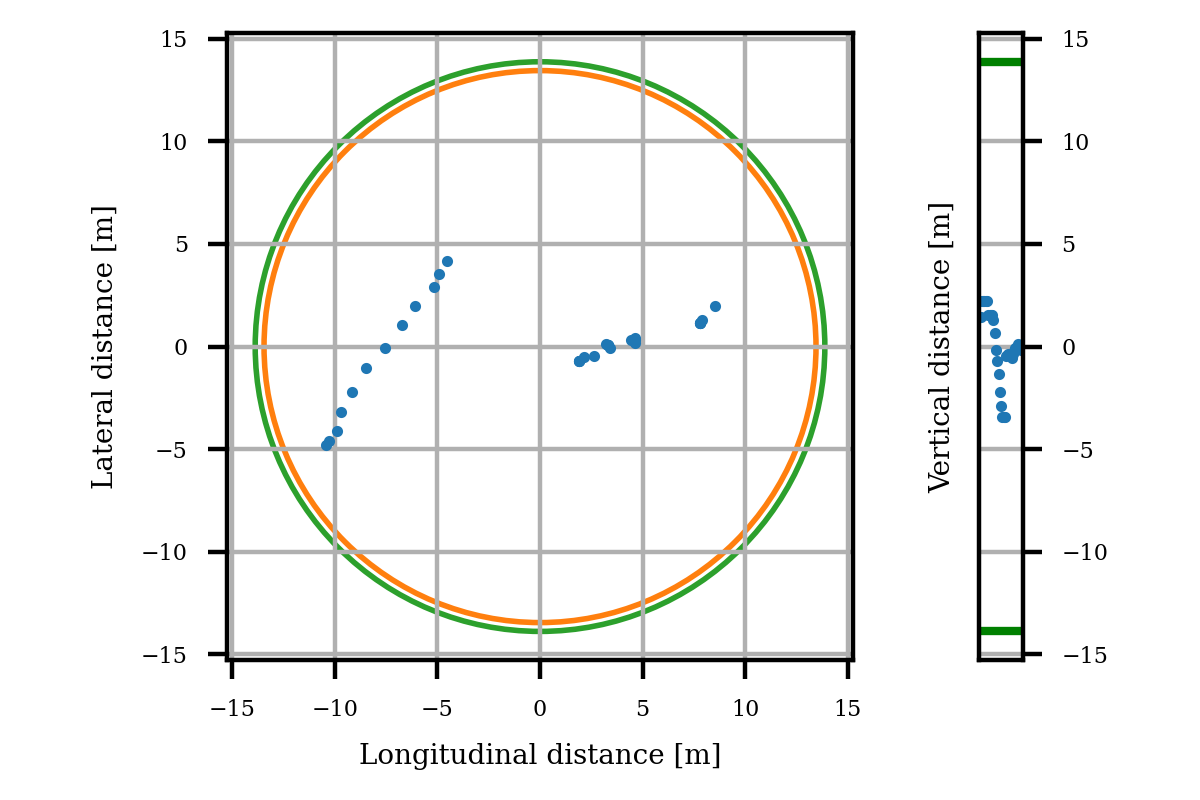
\includegraphics[width=\textwidth]{Static/raw_static_IPhone 11 Pro.png}
		      	  	\caption{Raw data}
		     	\end{subfigure}
		     	\begin{subfigure}[b]{0.45\textwidth}
		      	   \centering
		      	   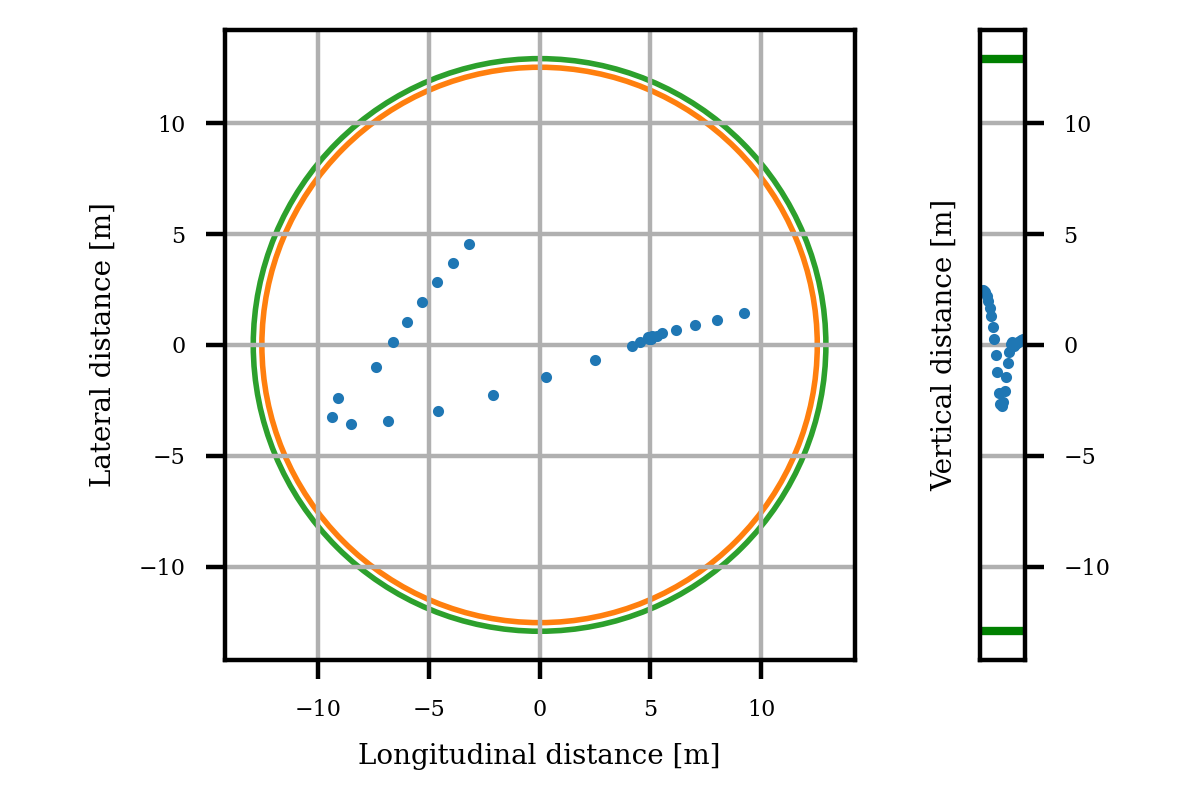
\includegraphics[width=\textwidth]{Static/cond_static_IPhone 11 Pro.png}
		      	   \caption{Conditioned data}
		     	\end{subfigure} 	
		      \caption{Position recording of iPhone 11 Pro}
		      \label{fig:static_loc_iPhone}
			\end{figure}		
			\begin{figure}[h]
		   		\centering
		     	\begin{subfigure}[b]{0.45\textwidth}
		      		\centering
		      	  	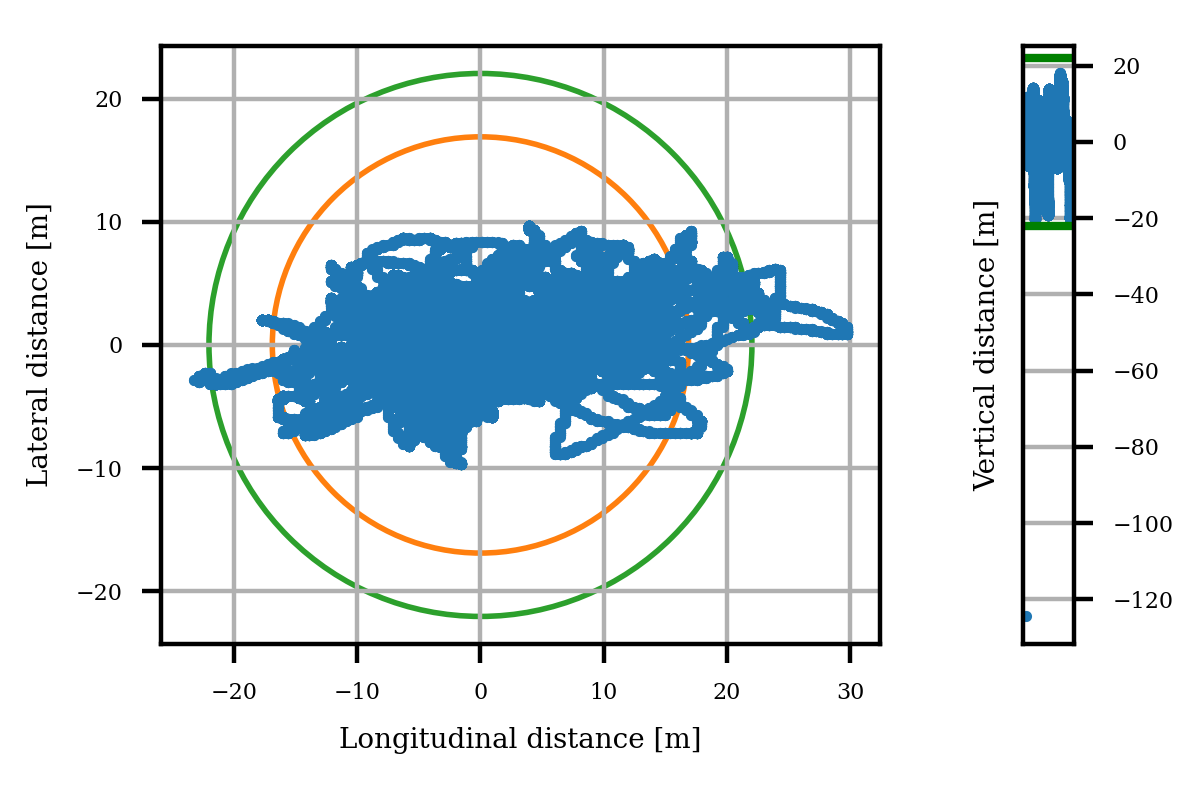
\includegraphics[width=\textwidth]{Static/raw_static_MTK 3339.png}
		      	  	\caption{Raw data}
		     	\end{subfigure}
		     	\begin{subfigure}[b]{0.45\textwidth}
		      	   \centering
		      	   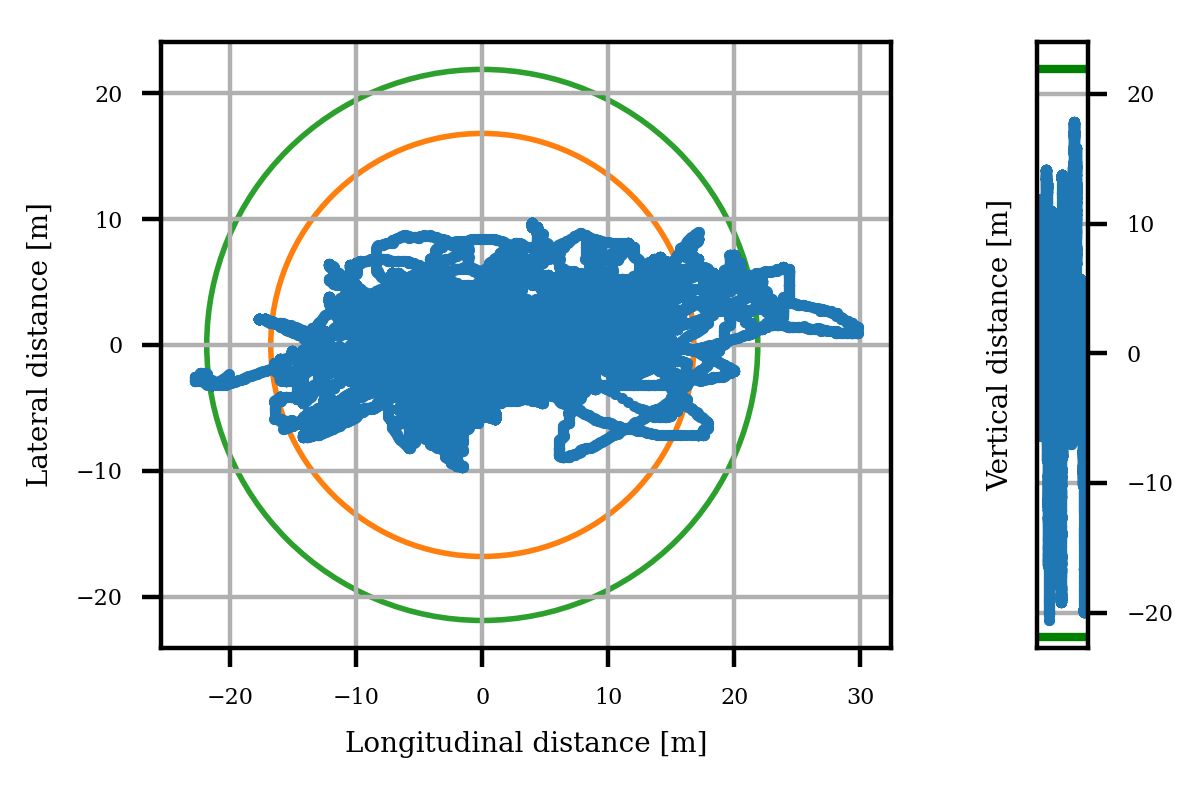
\includegraphics[width=\textwidth]{Static/cond_static_MTK 3339.png}
		      	   \caption{Conditioned data}
		     	\end{subfigure}
		      \caption{Position recording of U-blox M8N}
		      \label{fig:static_loc_gadget1}
			\end{figure}		
			\begin{figure}[h]
		   		\centering
		     	\begin{subfigure}[b]{0.45\textwidth}
		      		\centering
		      	  	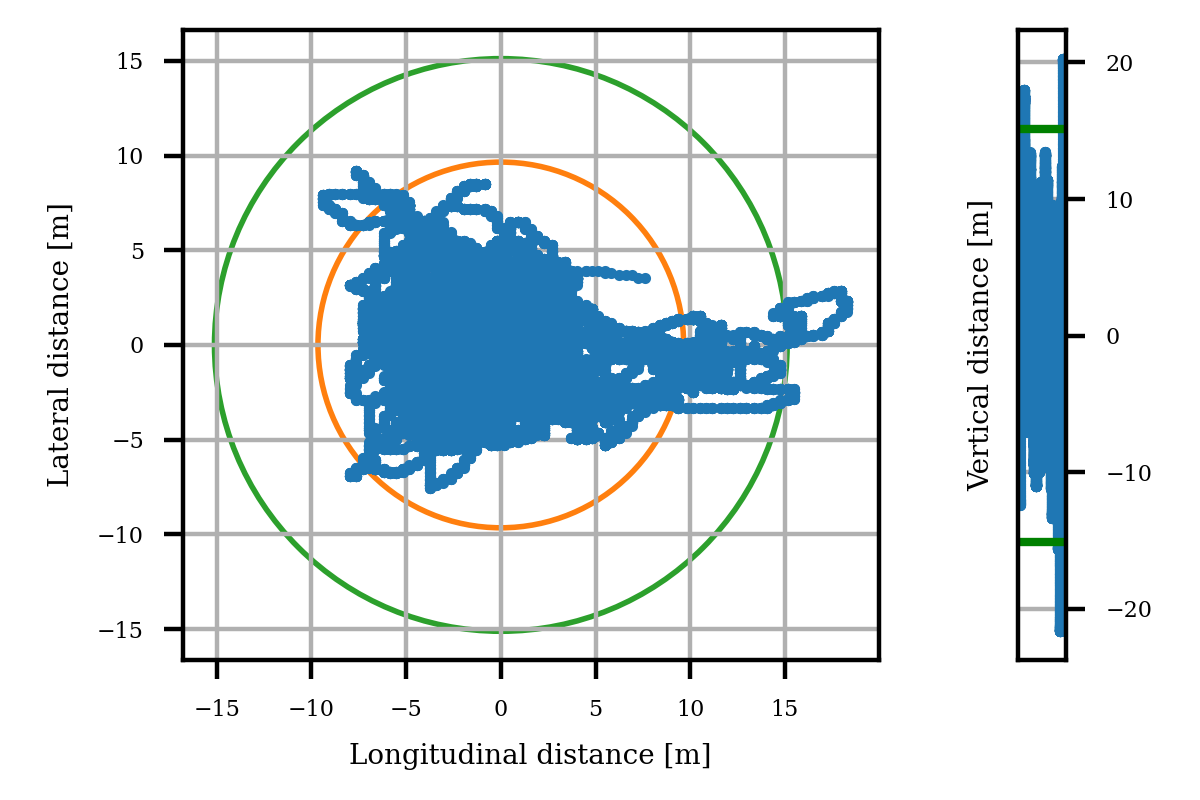
\includegraphics[width=\textwidth]{Static/raw_static_U-blox M8N.png}
		      	  	\caption{Raw data}
		     	\end{subfigure}
		     	\begin{subfigure}[b]{0.45\textwidth}
		      	   \centering
		      	   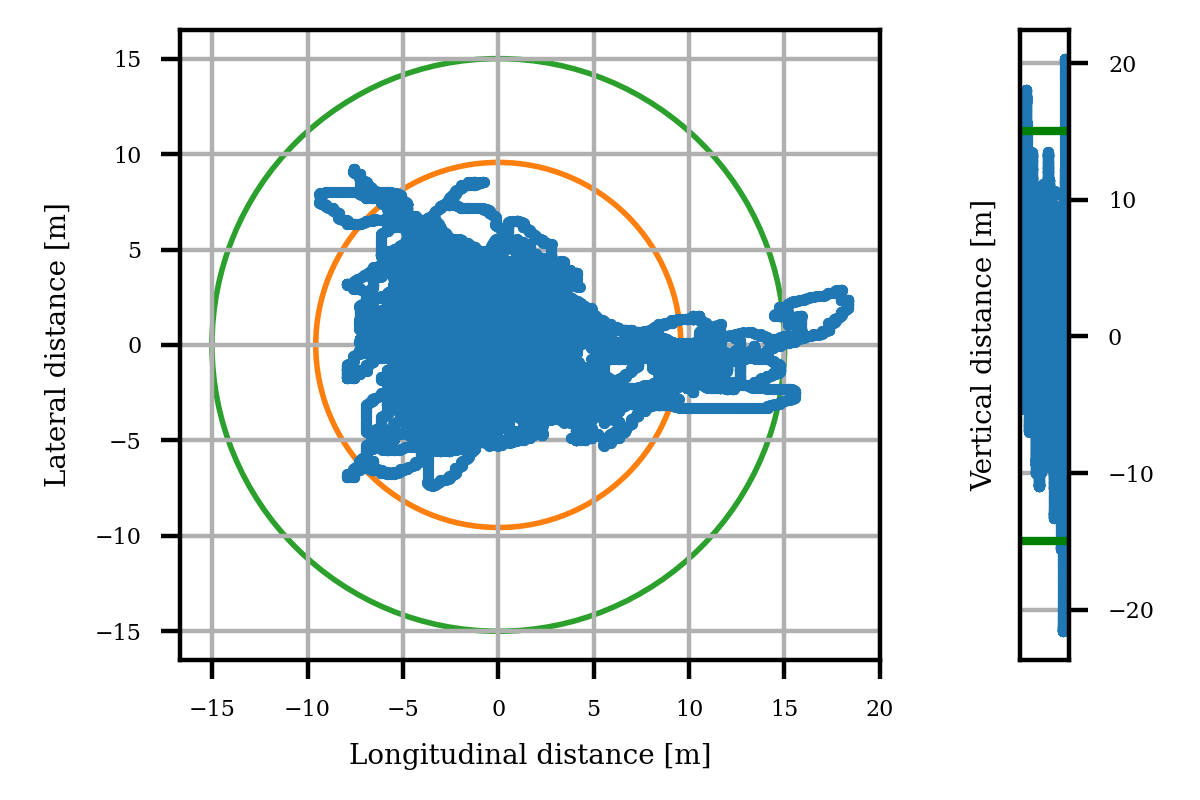
\includegraphics[width=\textwidth]{Static/cond_static_U-blox M8N.png}
		      	   \caption{Conditioned data}
		     	\end{subfigure}
		      \caption{Position recording of MTK 3339}
		      \label{fig:static_loc_gadget2}
			\end{figure}	
			Numerical results can be found in Table \ref{table:static_results}.
			\begin{table}[h]
				\centering
				\begin{tabular}{|c|c|c|c|c|}
					\hline 
					& \multicolumn{2}{c|}{Raw data} & \multicolumn{2}{c|}{Conditioned data} \\ 
					\hline 
					Equipment & R95 2D & R95 3D & R95 2D & R95 3D \\ 
					\hline 
					iPhone 11 Pro & 13.45 m & 13.88 m & 12.53 m & 12.92 m \\ 
					\hline 
					U-blox M8N & 9.65 m & 15.12 m & 9.57 m & 15.01 m \\ 
					\hline 
					MTK 3339 & 16.90 m & 22.04 m & 16.80 m & 21.88 m \\ 
					\hline 
				\end{tabular} 
			\caption{R95 values of static measurement}
			\label{table:static_results}
			\end{table}
			The calculated values of the iPhone can not be taken account due to the very low number of recorded points. For the Gadgets an increase between the 2D and 3D dimensional approach is seen due to the uncertainty of the altitude values. The U-blox M8N shows smaller radius values in all cases that shows higher accuracy of this device. The difference between the raw and conditioned dataset indicates that the data cleaning process is reducing the uncertainty while maintaining the same range of values. \\
			According to the device datasheets the horizontal accuracy of the U-blox M8N (MTK 3339 receiver) is claimed at 2.5 m. The reference value for MTK 3339 (U-blox M8N reciever) is stated at 3 m for 2DRMS by the datasheet which is equal for the R95 (2D) accuracy level. These values are not reached, current measurement exceeds these values by 7 to 15 meters. It has to be noted that such datasheet values are defined in measurements in clear condition and much longer period. Increasing measurement duration and selecting different test location most probably would increase the accuracy.\\
			The dilution of precision (DOP) and number of satellites after conditioning the data series is shown on Figure \ref{fig:static_dop_gadgets} except for the iPhone as no real data was recorded by the device.
			\begin{figure}[h]
		   		\centering
		     	\begin{subfigure}[b]{0.45\textwidth}
		      		\centering
		      	   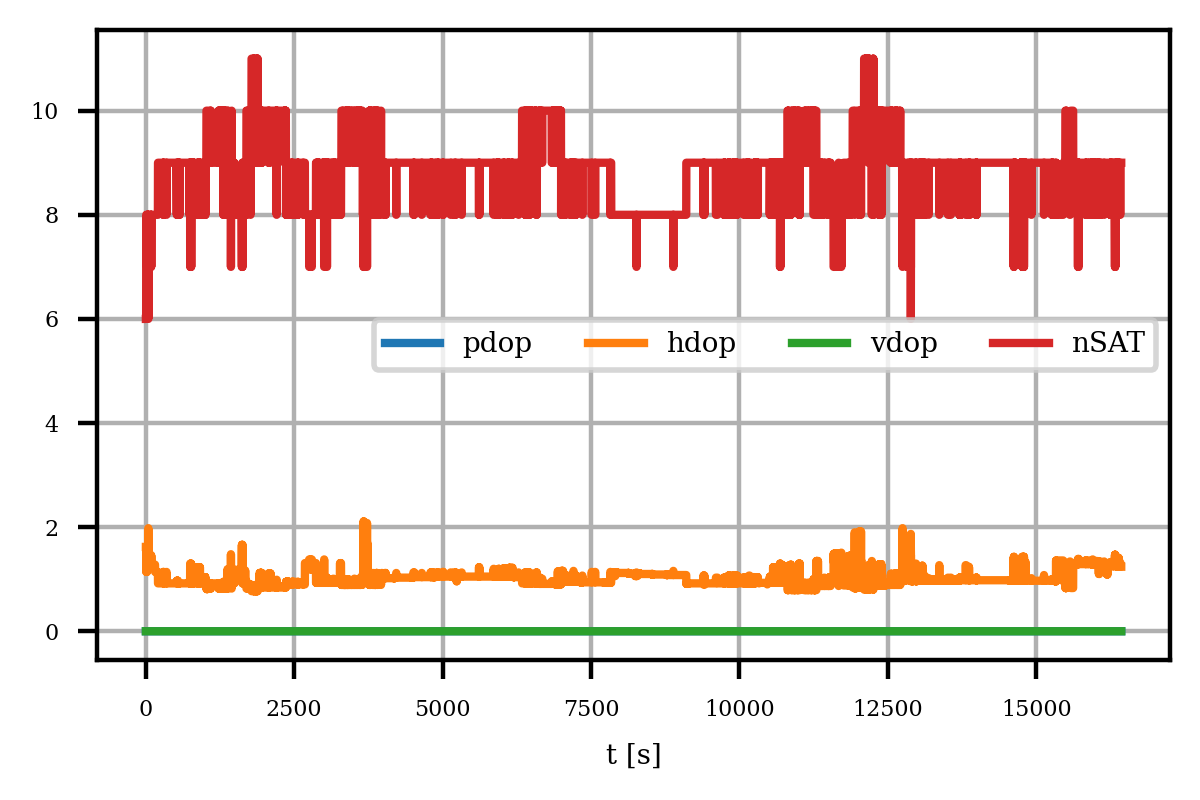
\includegraphics[width=\textwidth]{Static/cond_dop_MTK 3339.png}
		      	   \caption{U-blox M8N}
		     	\end{subfigure}
		     	\begin{subfigure}[b]{0.45\textwidth}
		      	   \centering
		      	   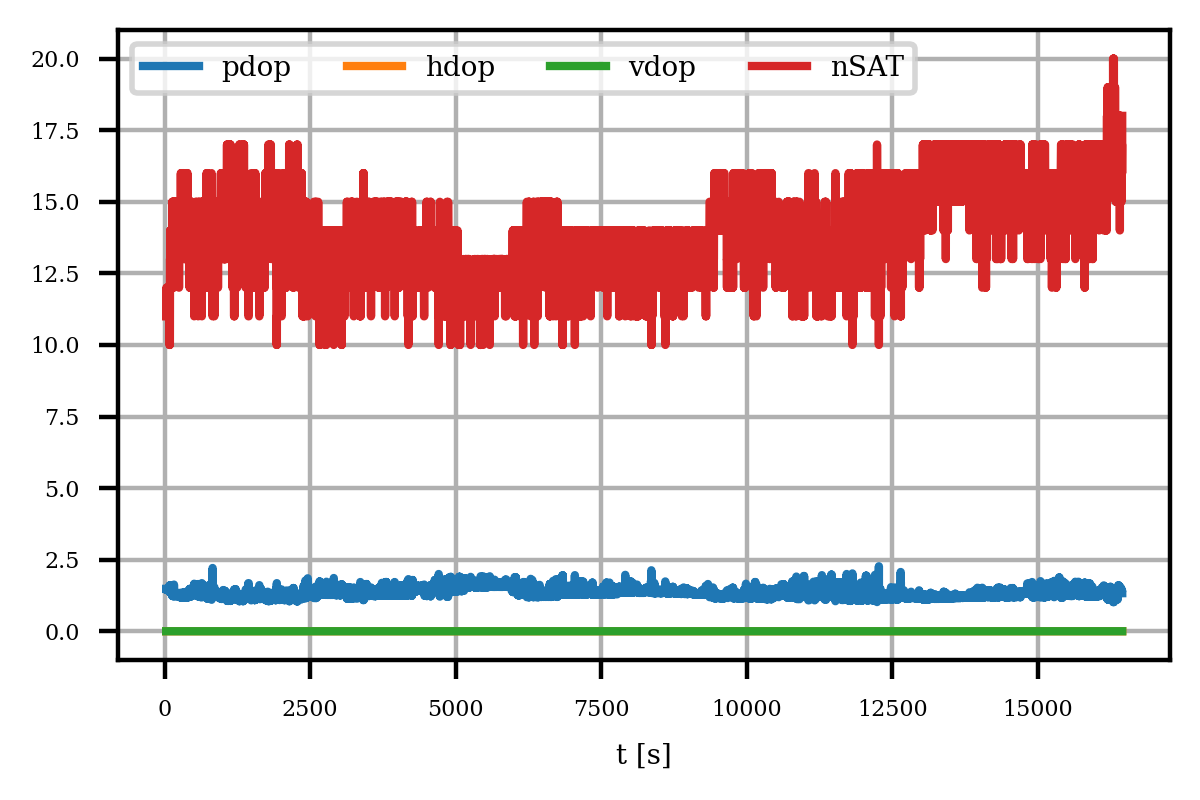
\includegraphics[width=\textwidth]{Static/cond_dop_U-blox M8N.png}
		      	   \caption{MTK 3339}
		     	\end{subfigure}
		      \caption{DOP and number of satellites - static testing}
		      \label{fig:static_dop_gadgets}
			\end{figure}
			U-blox M8N shows a positional DOP value ranging below 2.5, averaging at 1.34. MTK 3339 reaches a horizontal DOP below 2 with a mean value of 1.01. Both devices show excellent accuracy according to \cite{tahsinAnalysisDOPIts2015}. This is also proved by the number of satellites which changes between 10 and 20 for U-blox M8N and between 6 and 11 for MTK 3339.
			
		\subsection{Dynamic test}
			The dynamic test was held on 28th of November, 2021 on the highway M6 between cities of Budapest and Dunaföldvár. The route leads through a plain area with low obstacles in the way of the GNSS signals, therefore it provides fairly good possibilities for GNSS system tests, however on the given day heavy rain was experienced that might limit the quality of the signals. Seven speed steps were taken from 70 km/h up to 130 km/h and then down to 80 km/h, at each step maintaining the speed at around 2 to 3 kilometers. The resulting speed and altitude profile is presented on Figure \ref{fig:dynamic_speed} and Figure \ref{fig:dynamic_alt}. \\
			The raw measurement data holds 1351 datapoints for the iPhone 11 Pro, and 6749 and 13528 points for the U-blox M8N and 2 respectively. After performing the data cleaning 87, 605 and 468 points removed, leading to a loss of 12,9\%, 8,9\% and 3,5\% compared to the number of raw datapoints. During this process the outliers successfully removed and the characteristics of each curves are maintained. \\
			The difference of approximately 4 km/h between the cruise control speed and the measured real speed can be identified. In case of the speed profile a clear deviation of MTK 3339 from the other two devices can be seen, there is an offset in the curves showing that the speed profile is delayed with approximately one step. Such deviation can not be found on the altitude graphs. The effect of this behaviour is most probably a delayed update of the speed values. Similar behaviour can be identified in the detailed inspection of the recorded data, the same speed data is stored for each step and no fluctuation of the value is observed. This is also represented during the calculation of speed characteristics, where the standard deviation shows a very low variability of the speed values for each speed step. Please refer to Table \ref{table:dyn_speed_raw} and \ref{table:dyn_speed_conditioned} \\			
			Comparing the altitude recordings the U-blox M8N recorded the lowest and MTK 3339 the highest values, while the iPhone recorded the altitude mostly in between.. All three devices show very similar elevation profiles, the maximum deviation between the curves are not exceeding 6 meters. \\
			The smoothness of the curves are different for each devices, in case of the iPhone a more noisy signal is obtained indicating higher uncertainty in the recordings, while the U-blox M8N provided a relatively smooth series with low variation and MTK 3339 resulted in even more smoother recordings. In case of the MTK 3339 the detailed view on the recorded data revealed once again that the parameters are often held for several seconds between each updates. This implies that the sampling frequency of 10 Hz is jeopardized by the update rates of the single parameters (so called update of the GNSS fixes).
			\begin{figure}[h]
		   		\centering
		     	\begin{subfigure}[b]{0.45\textwidth}
		      		\centering
		      	  	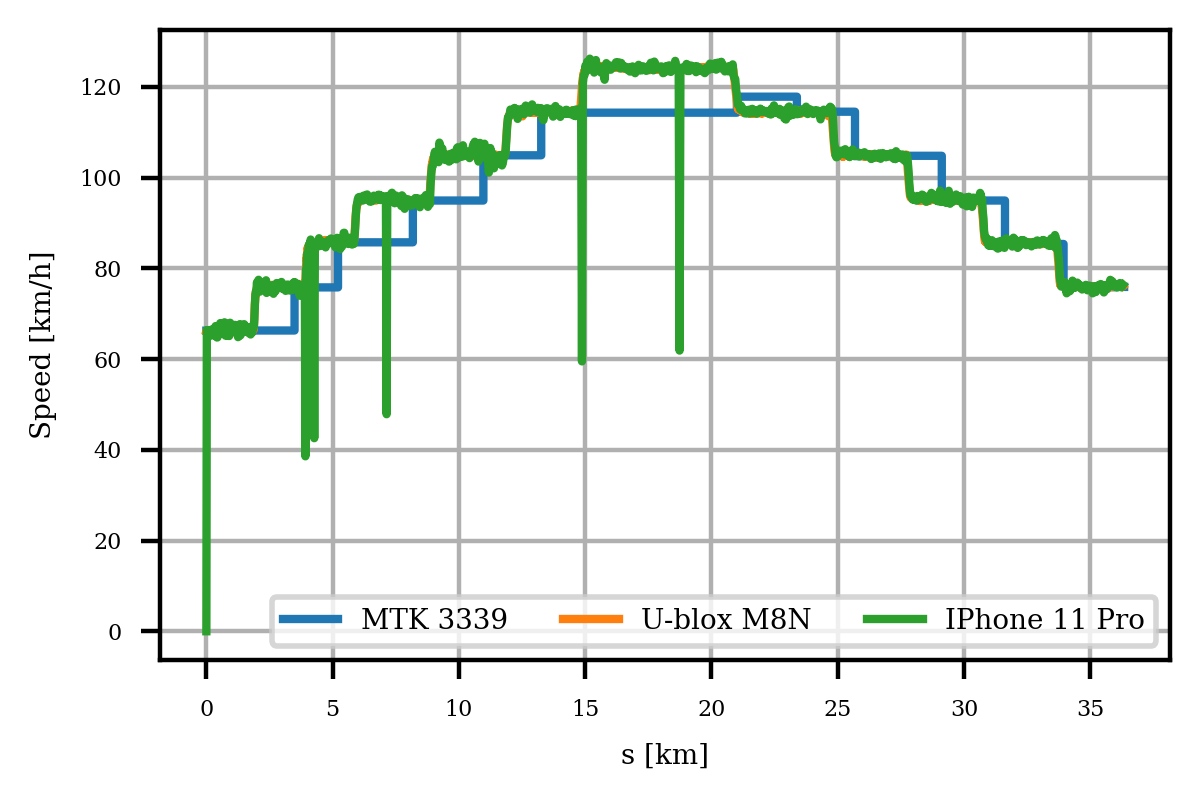
\includegraphics[width=\textwidth]{Dynamic/raw_speed.png}
		      	  	\caption{Raw data}
		     	\end{subfigure}
		     	\begin{subfigure}[b]{0.45\textwidth}
		      	   \centering
		      	   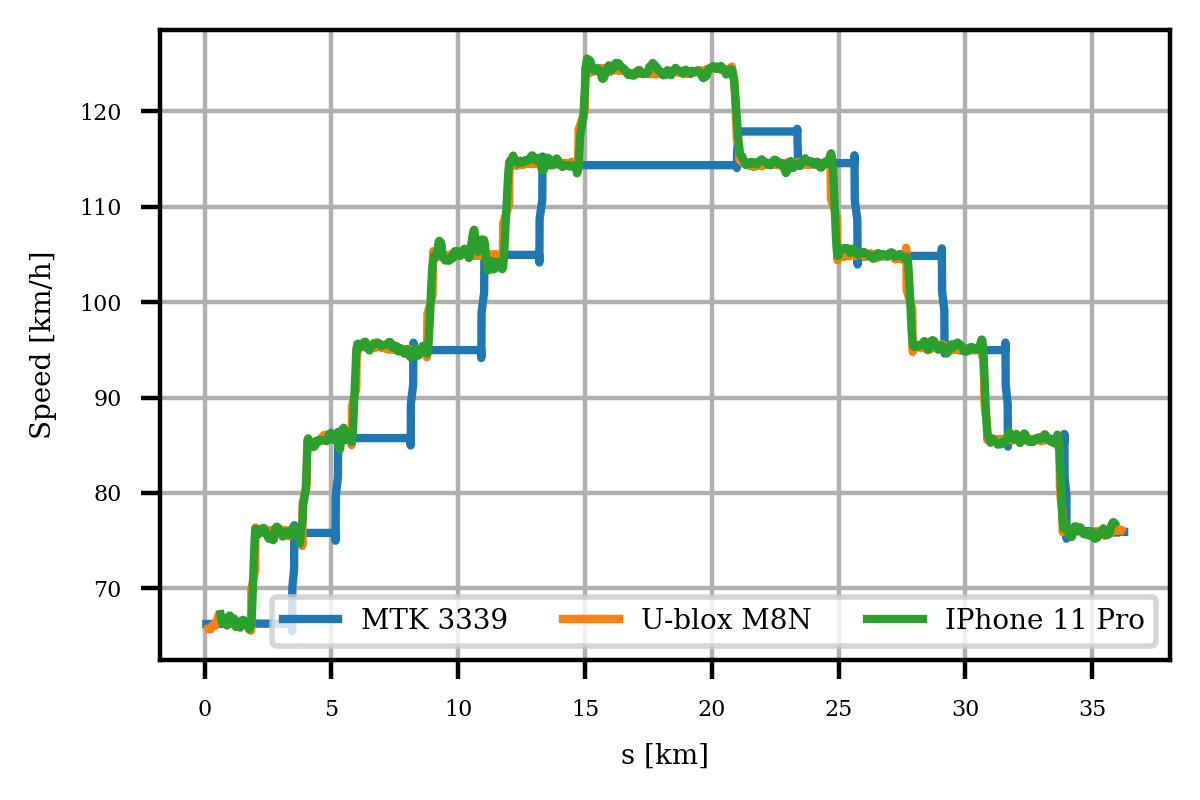
\includegraphics[width=\textwidth]{Dynamic/cond_speed.png}
		      	   \caption{Conditioned data}
		     	\end{subfigure}
		     	
		      \caption{Speed recordings of the receivers during dynamic testing}
		      \label{fig:dynamic_speed}
			\end{figure}		
			\begin{figure}[h]
		   		\centering
		     	\begin{subfigure}[b]{0.45\textwidth}
		      		\centering
		      	  	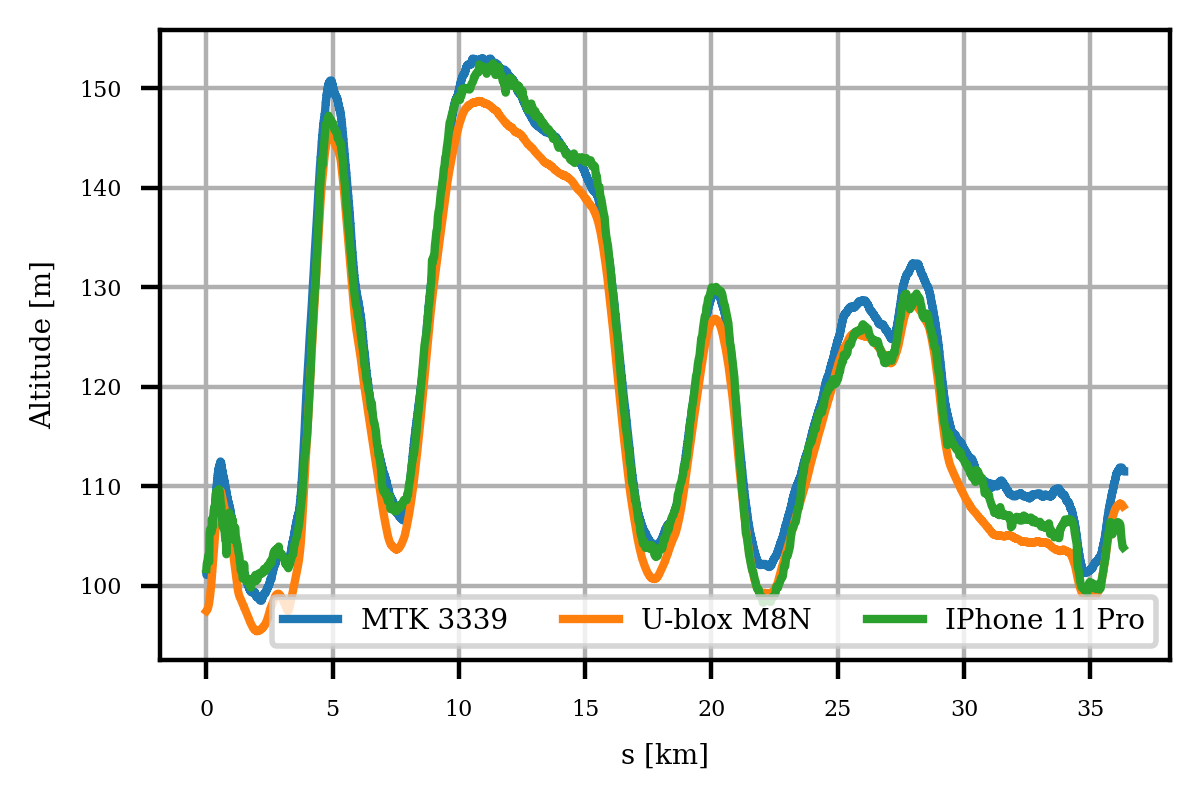
\includegraphics[width=\textwidth]{Dynamic/raw_alt.png}
		      	  	\caption{Raw data}
		     	\end{subfigure}
		     	\begin{subfigure}[b]{0.45\textwidth}
		      	   \centering
		      	   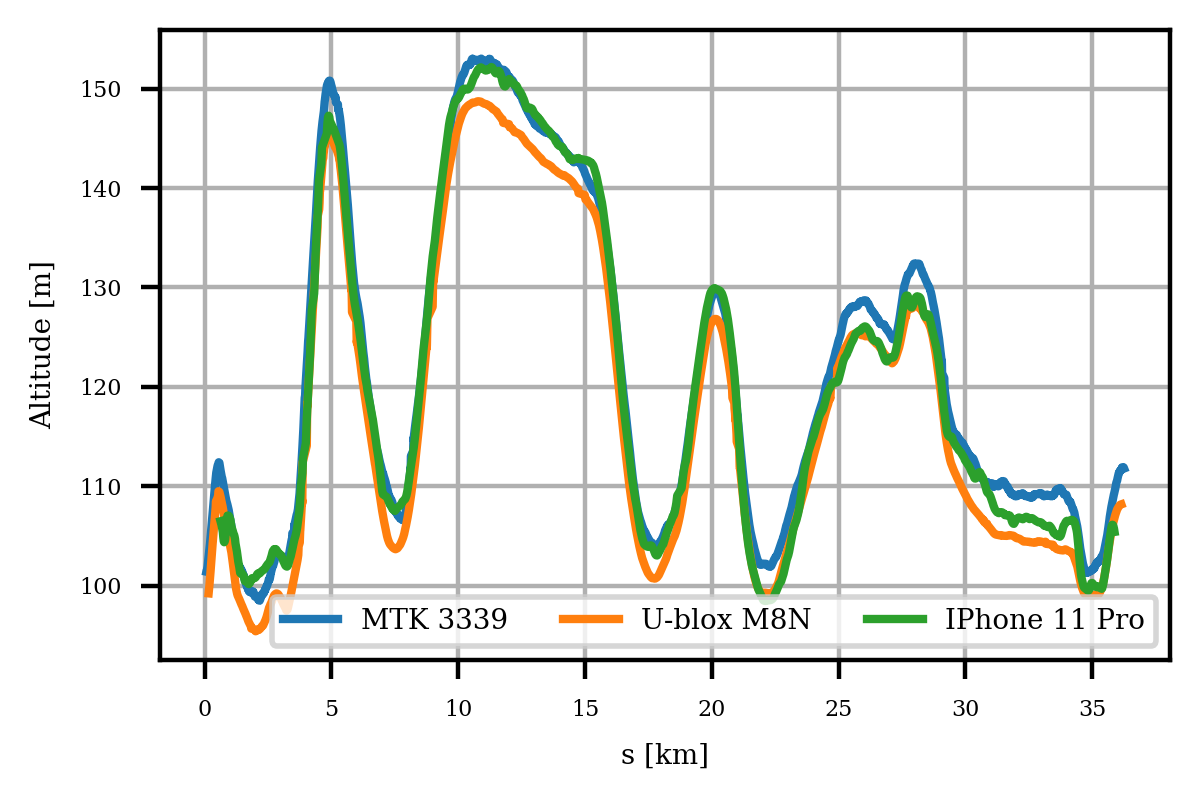
\includegraphics[width=\textwidth]{Dynamic/cond_alt.png}
		      	   \caption{Conditioned data}
		     	\end{subfigure}
		     	
		      \caption{Altitude recordings of the receivers during dynamic testing}
		      \label{fig:dynamic_alt}
			\end{figure}	
			
			The calculation of the mean speed values and their standard deviation can be found in Table \ref{table:dyn_speed_raw} and Table \ref{table:dyn_speed_conditioned}.
			\begin{table}[h]
			\centering
				\begin{tabular}{|c|c|c|c|c|c|c|c|c|c|c|c|c|}
				\hline 
				& \multicolumn{2}{c|}{iPhone 11 Pro} & \multicolumn{2}{c|}{U-blox M8N} & \multicolumn{2}{c|}{MTK 3339} \\ 
				\hline 
				Cruise control speed & Mean & St. dev. & Mean & St. dev & Mean & St. dev \\ 
				\hline 
				70 & 66.39 & 0.94 & 66.41 & 0.39 & 66.30 & 0.01 \\ 
				\hline 
				80 & 75.96 & 0.77 & 75.92 & 0.54 & 75.88 & 0.07 \\ 
				\hline 
				90 & 85.61 & 0.83 & 85.61 & 0.71 & 85.65 & 0.11 \\ 
				\hline 
				100 & 95.26 & 0.84 & 95.13 & 0.62 & 95.02 & 0.14 \\ 
				\hline 
				110 & 104.99 & 1.13 & 104.86 & 0.63 & 104.86 & 0.06 \\ 
				\hline 
				120 & 114.61 & 0.80 & 114.49 & 0.65 & 115.09 & 1.37 \\ 
				\hline 
				130 & 124.18 & 0.75 & 124.10 & 0.44 & NA & NA \\ 
				\hline 
				\end{tabular} 
			\caption{Speed results of dynamic testing - raw data in km/h}
			\label{table:dyn_speed_raw}			
			\end{table}
			\begin{table}[h]
				\centering
				\begin{tabular}{|c|c|c|c|c|c|c|c|c|c|c|c|c|}
				\hline 
				& \multicolumn{2}{c|}{iPhone 11 Pro} & \multicolumn{2}{c|}{U-blox M8N} & \multicolumn{2}{c|}{MTK 3339} \\ 
				\hline 
				Cruise control speed & Mean & St. dev. & Mean & St. dev & Mean & St. dev \\ 
				\hline 
				70 & 66.56 & 0.56 & 66.40 & 0.34 & 66.30 & 0.05 \\ 
				\hline 
				80 & 75.91 & 0.66 & 75.92 & 0.31 & 75.88 & 0.23 \\ 
				\hline 
				90 & 85.61 & 0.87 & 85.65 & 0.45 & 85.66 & 0.22 \\ 
				\hline 
				100 & 95.28 & 0.81 & 95.14 & 0.38 & 95.02 & 0.24 \\ 
				\hline 
				110 & 105.01 & 0.93 & 104.88 & 0.31 & 104.86 & 0.21 \\ 
				\hline 
				120 & 114.63 & 0.83 & 114.48 & 0.39 & 115.09 & 1.38 \\ 
				\hline 
				130 & 124.20 & 0.55 & 124.14 & 0.33 & NA & NA \\ 
				\hline 
				\end{tabular} 
			\caption{Speed results of dynamic testing - conditioned data in km/h}
			\label{table:dyn_speed_conditioned}
			\end{table}
			The calculated mean values for the speed steps are identical in the range of the whole part. After conditioning the data the mean values change in the decimals and hundredths only. The standard deviation are different for the three devices. The iPhone shows the largest values ranging up to 0.93 km/h after data conditioning. The U-blox M8N shows a deviation up to 0.45 km/h and the MTK 3339 reaches 1.38 km/h. For the latter in all cases except one the standard deviation is below 0.24 km/h. Due to the slow update of the GNSS fixes for the MTK 3339 these accuracy measures are questionable. Further measurements are needed to analyze whether such low values can be achieved or not. Besides that the U-blox M8N shows higher accuracy than the iPhone. The effect of the data conditioning can be also observed as the mean values are unaffected but the standard deviation values are greatly reduced while keeping approximately 90\% of the measurement points. Calculation results for MTK 3339 for the speed step of 130 km/h is not available due to the missing update from the receiver. \\
			Dilution of precision and satellite information is shown on Figure \ref{fig:dyn_dop_gadgets} and Figure \ref{fig:dyn_dop_iphone}.
			\begin{figure}[h]
		   		\centering
		     	\begin{subfigure}[b]{0.45\textwidth}
		      		\centering
		      	   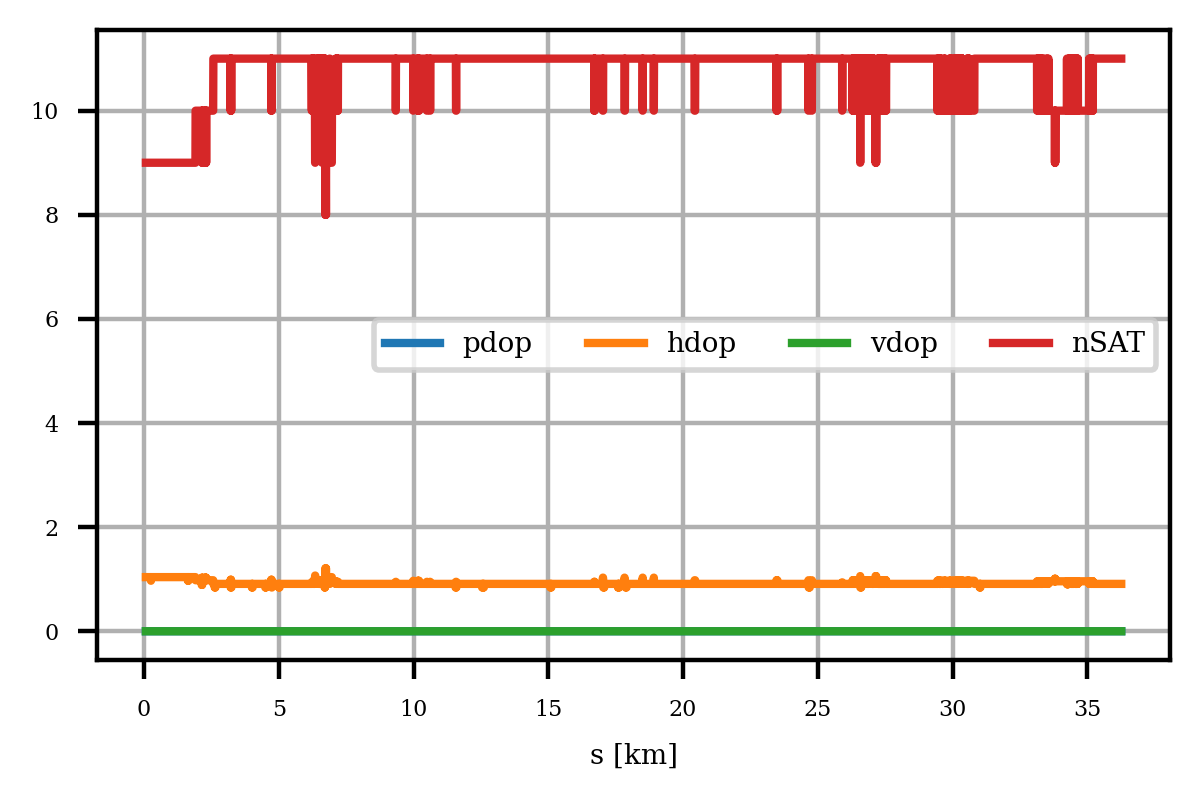
\includegraphics[width=\textwidth]{Dynamic/cond_dop_MTK 3339.png}
		      	   \caption{U-blox M8N}
		      	   \label{fig:dyn_dop_gadget1}
		     	\end{subfigure}
		     	\begin{subfigure}[b]{0.45\textwidth}
		      	   \centering
		      	   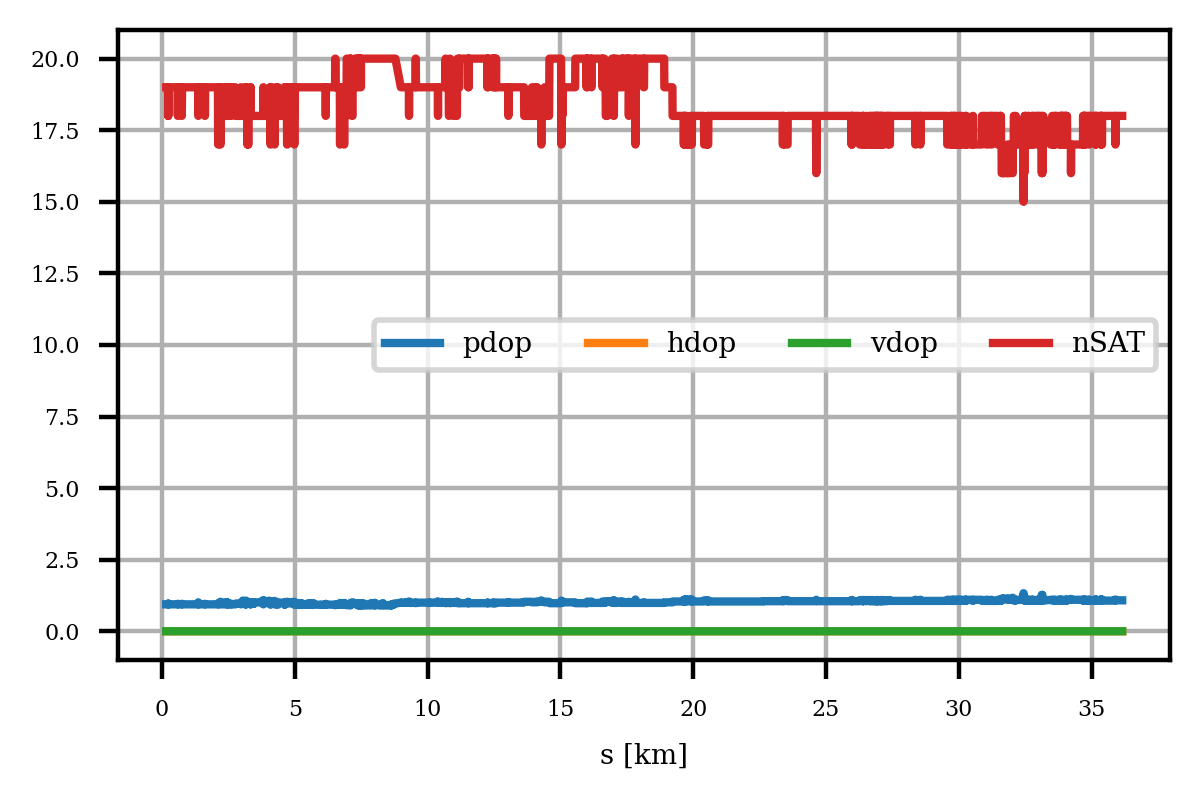
\includegraphics[width=\textwidth]{Dynamic/cond_dop_U-blox M8N.png}
		      	   \caption{MTK 3339}
		      	   \label{fig:dyn_dop_gadget2}
		     	\end{subfigure}
		      \caption{DOP and number of satellites - dynamic testing}
		      \label{fig:dyn_dop_gadgets}
			\end{figure}
			\begin{figure}[h]
		   		\centering
		     	\begin{subfigure}[b]{0.45\textwidth}
		      		\centering
		      	   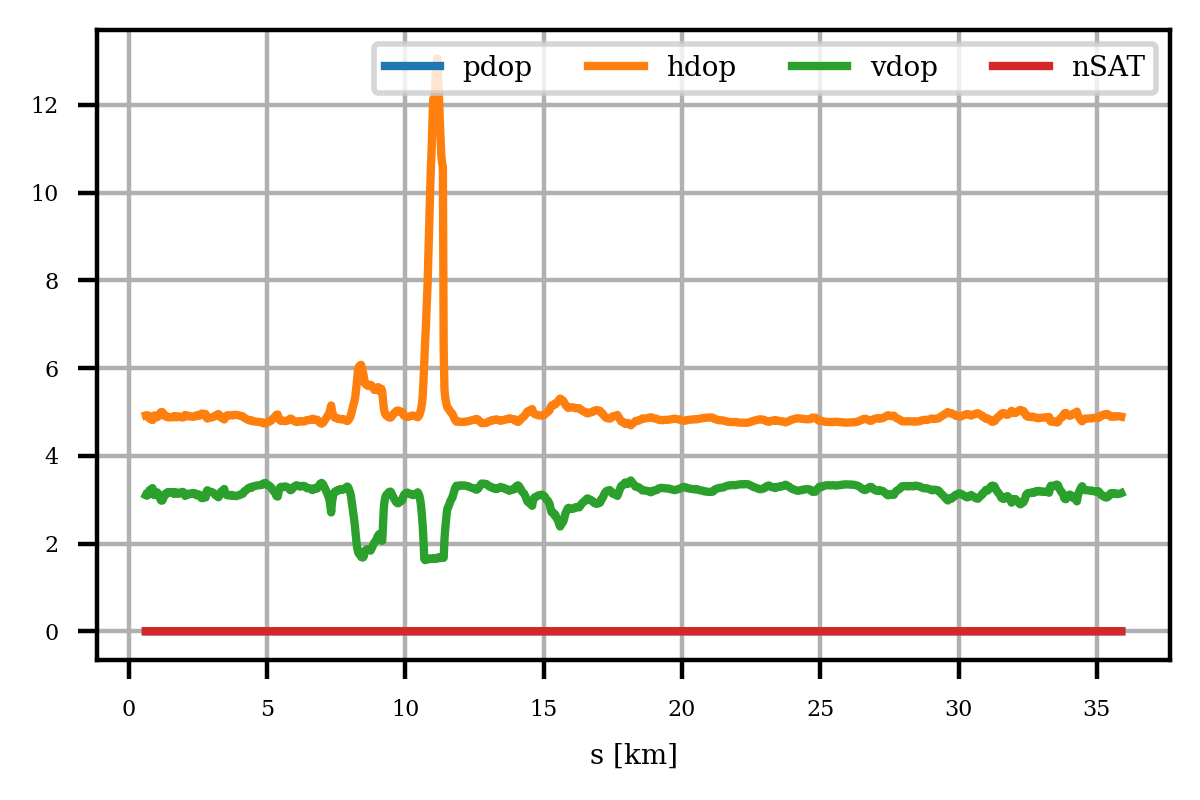
\includegraphics[width=\textwidth]{Dynamic/cond_dop_IPhone 11 Pro.png}
		     	\end{subfigure}
				\caption{DOP and number of satellites - dynamic testing - iPhone 11 Pro}		     	
		      \label{fig:dyn_dop_iphone}
			\end{figure}
			The positional DOP value for U-blox M8N shows high accuracy as it stays below 2, having a mean of 1.018. MTK 3339 reaches a horizontal DOP value of 0.928 on average. The iPhone 11 Pro measurement results in a mean of horizontal DOP value of 5.00 and a vertical DOP value of 3.10. The number of satellites ranges between 15 and 20, 8 and 11 for U-blox M8N and MTK 3339 and not recorded for the iPhone. These results show excellent accuracy of U-blox M8N and MTK 3339 and good accuracy for the iPhone 11 Pro.
			
		\subsection{Route profile}
			A single route profile for the assessment is selected starting at Füzesabony station, heading to Budapest-Keleti station. The route section in this case starts at the plain section then approaching the hilly area of Gödöllő and arriving to the urban city of Budapest. The location raw and conditioned data is presented on Figure \ref{fig:route_map}. Unfortunately during the measurement MTK 3339 produced a failure in the software which resulted in no data logging, therefore the current analysis focuses only on iPhone and U-blox M8N. \\
			The iPhone recorded 5574 datapoints and during conditioning 789 points were removed resulting to a dataloss of 14\%. The U-blox M8N recorded 29186 datapoints from which 1671 was removed leading to a loss of 5,7\%. It can be seen that the raw data provided a good tracking of the position over the full route profile. The iPhone location data was not so accurate as the recordings with U-blox M8N, especially on the second section at Gödöllő Hills, a clear deviation of the route can be observed. After data cleansing and filtering as the less accurate points were removed the location of the iPhone show larger deviation compared to the recordings of U-blox M8N. Both for the iPhone and U-blox M8N the first and third section, the urban area and the plain area respectively resulted in a comparable tracking of the location with limited differences of the location information and higher deviation is observed in the hilly area of Gödöllő. The receivers found the satellite signals in a couple of minutes and there was no loss of signal experienced.
			\begin{figure}[h]
				\centering
				\begin{subfigure}[b]{0.45\textwidth}
					\centering
			      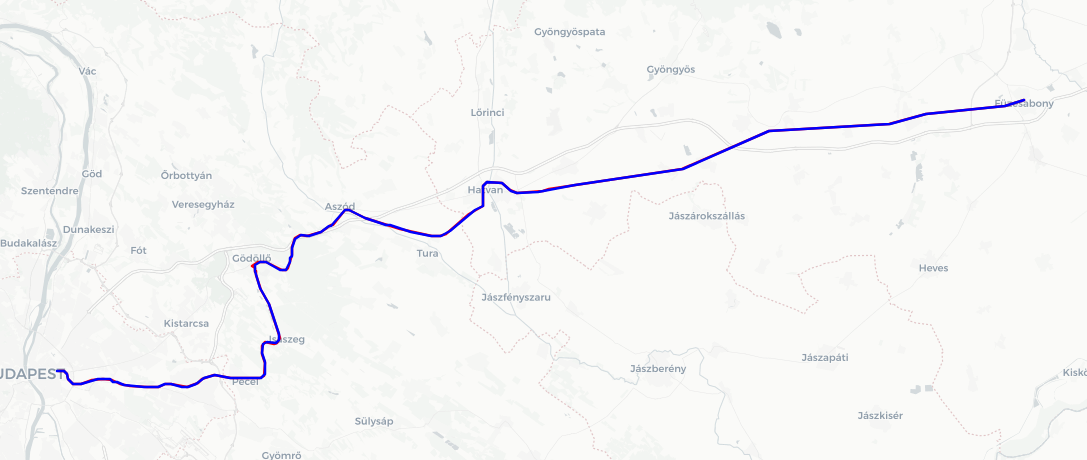
\includegraphics[width=\textwidth]{raw_map.png}
			      \caption{Raw data}
				\end{subfigure}
				\begin{subfigure}[b]{0.45\textwidth}
					\centering
			      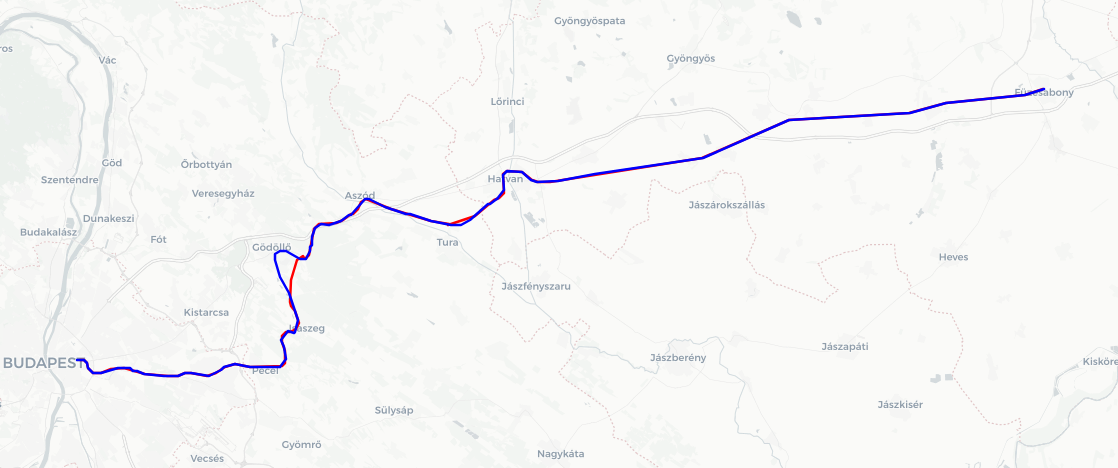
\includegraphics[width=\textwidth]{cond_map.png}
			      \caption{Conditioned data}
				\end{subfigure}
		   \caption{Position from route profile recording}
		   \begin{tabular}{c c}
				\footnotesize (Red - iPhone 11 Pro & \footnotesize Blue - U-blox M8N)
	      \end{tabular} 
		   \label{fig:route_map}
			\end{figure}

			Altitude data before and after the data conditioning algorithm is shown in Figure \ref{fig:route_alt}. Clear difference between the recordings of iPhone and U-blox M8N can be observed. The iPhone supplied data with much less variation while the recordings of the U-blox M8N varies in a much bigger interval greatly exceeding the usual gradients of the railway track. Removing the outliers and filtering the dataset the graph became more smooth, the variation of the U-blox M8N data is reduced. Similar effect was observed for the iPhone recording. Additionally the top of the Gödllő Hills, the peak of the altitude is removed from the iPhone dataset. Variation of the U-blox M8N dataset has the same trend that was recorded with the iPhone.
			\begin{figure}[h]
		   		\centering
		     	\begin{subfigure}[b]{0.45\textwidth}
		      		\centering
		      	  	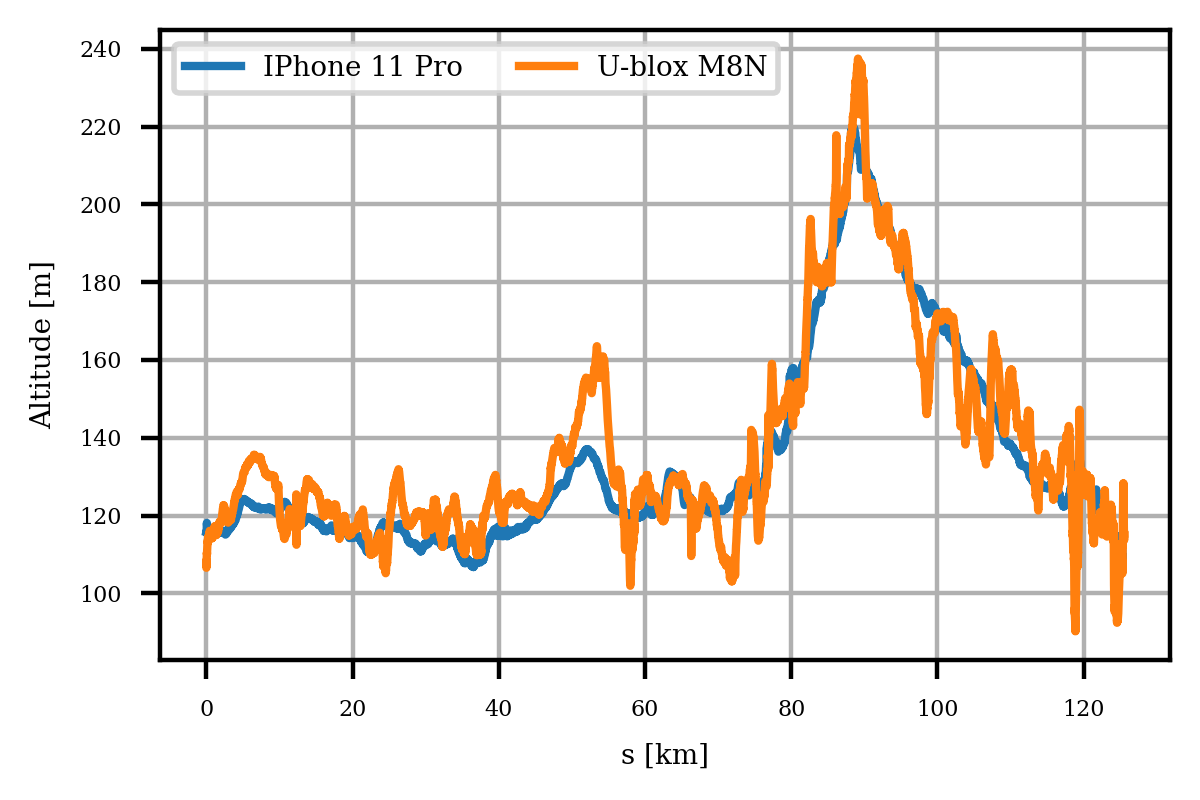
\includegraphics[width=\textwidth]{Route/raw_alt.png}
		      	  	\caption{Raw data}
		     	\end{subfigure}
		     	\begin{subfigure}[b]{0.45\textwidth}
		      	   \centering
		      	   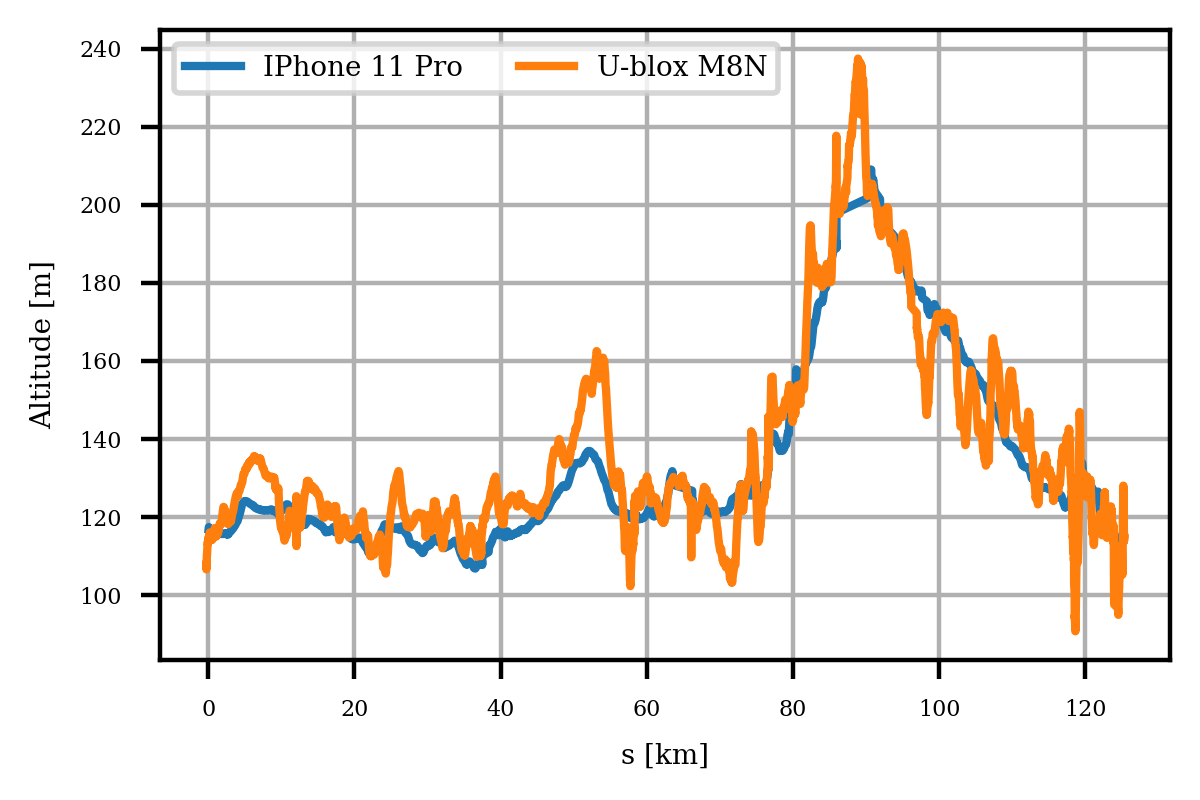
\includegraphics[width=\textwidth]{Route/cond_alt.png}
		      	   \caption{Conditioned data}
		     	\end{subfigure}
			   \caption{Altitude recording from route profile}
			   \label{fig:route_alt}
		   \end{figure}

			The registered speed values for the raw and conditioned data is shown on Figure \ref{fig:route_speed}. On the raw data several outliers can be identified that are exceeding the vehicle maximum speed (160 km/h) and the allowed maximum speed of the tracks (120 km/h). The outliers belong to the data recorded by the iPhone, while the U-blox M8N contains data only in the valid speed range. After removing these data and applying the Savitzky-Golay filter, the speed profile is obtained. Well corresponding signals can be seen however some observations can be done. All ten stations can be identified for U-blox M8N while iPhone 11 misses some of them especially after the data conditioning. At some points, where the outliers have been removed the speed profile is also lost. This concentrates on the Gödöllő Hills part of the second section of the route. Some phase shifting can be seen between the two tools towards the end of the recorded profile that corresponds to the urban area of Budapest. On the plain area (which is in this case the beginning of the route) good correlation between the signals of the devices can be sseen.
			\begin{figure}[h]
		   		\centering
		     	\begin{subfigure}[b]{0.45\textwidth}
		      		\centering
		      	  	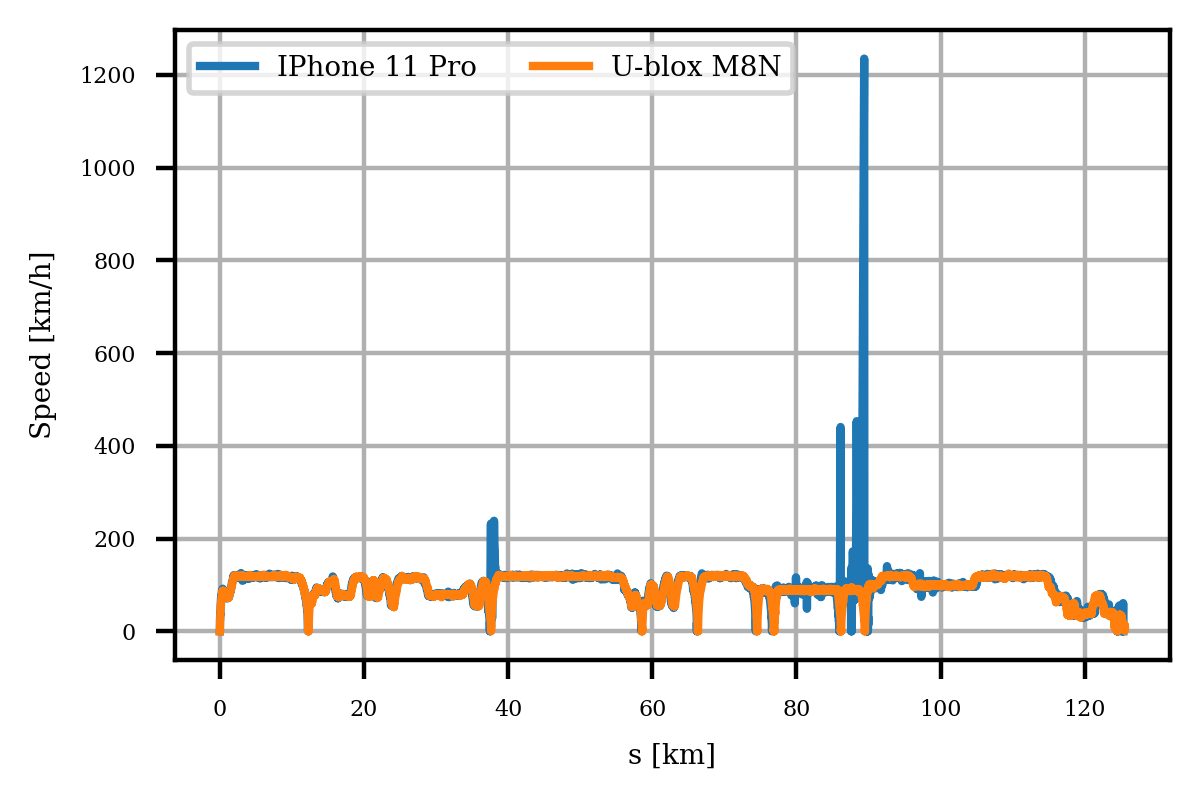
\includegraphics[width=\textwidth]{Route/raw_speed.png}
		      	  	\caption{Raw data}
		     	\end{subfigure}
		     	\begin{subfigure}[b]{0.45\textwidth}
		      	   \centering
		      	   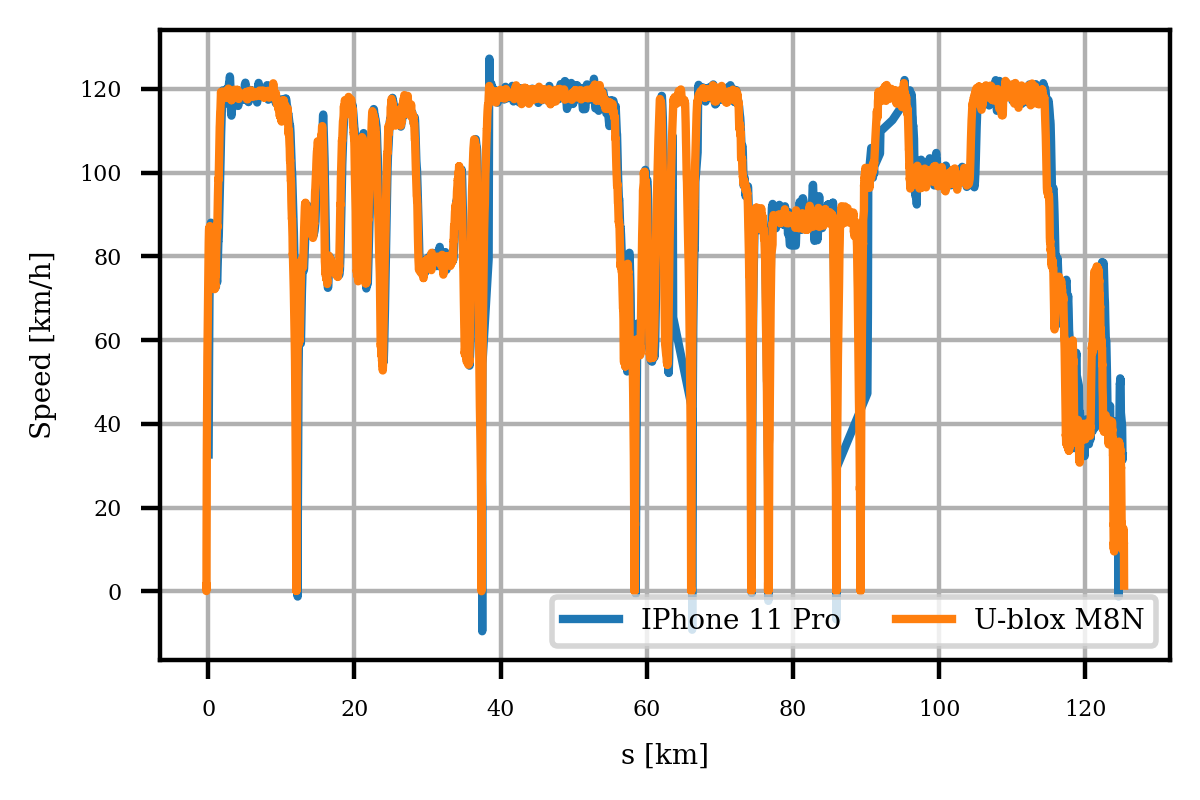
\includegraphics[width=\textwidth]{Route/cond_speed.png}
		      	   \caption{Conditioned data}
		     	\end{subfigure}
			   \caption{Speed recording from route profile}
			   \label{fig:route_speed}
		   \end{figure}

			In order to describe the accuracy of the measurements the dilution of precision (DOP) values and the number of satellites are presented in Figure \ref{fig:iPhone_dop} and Figure \ref{fig:Gadget1_dop}. 
			
			\begin{figure}[h]
		   		\centering
		     	\begin{subfigure}[b]{0.45\textwidth}
		      		\centering
		      	   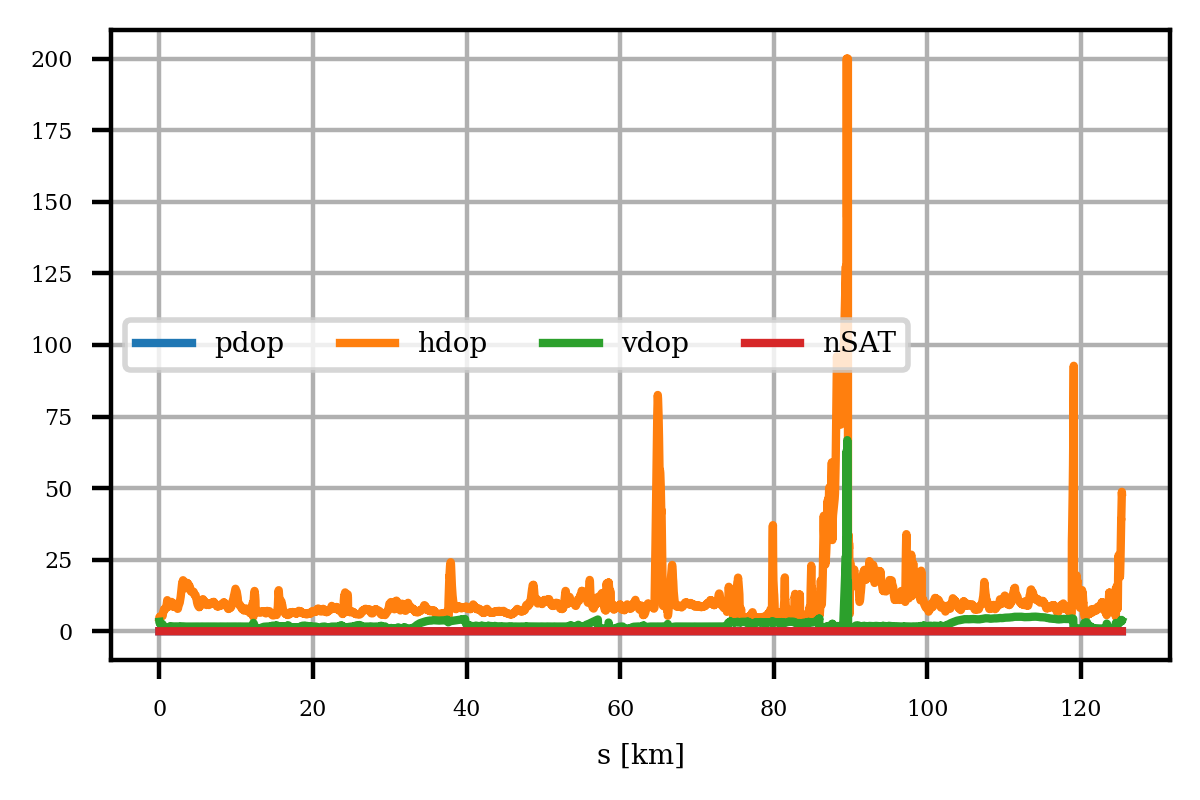
\includegraphics[width=\textwidth]{Route/raw_dop_IPhone 11 Pro.png}
		      	   \caption{Raw data}
		      	   \label{fig:iPhone_raw_dop}
		     	\end{subfigure}
		     	\begin{subfigure}[b]{0.45\textwidth}
		      	   \centering
		      	   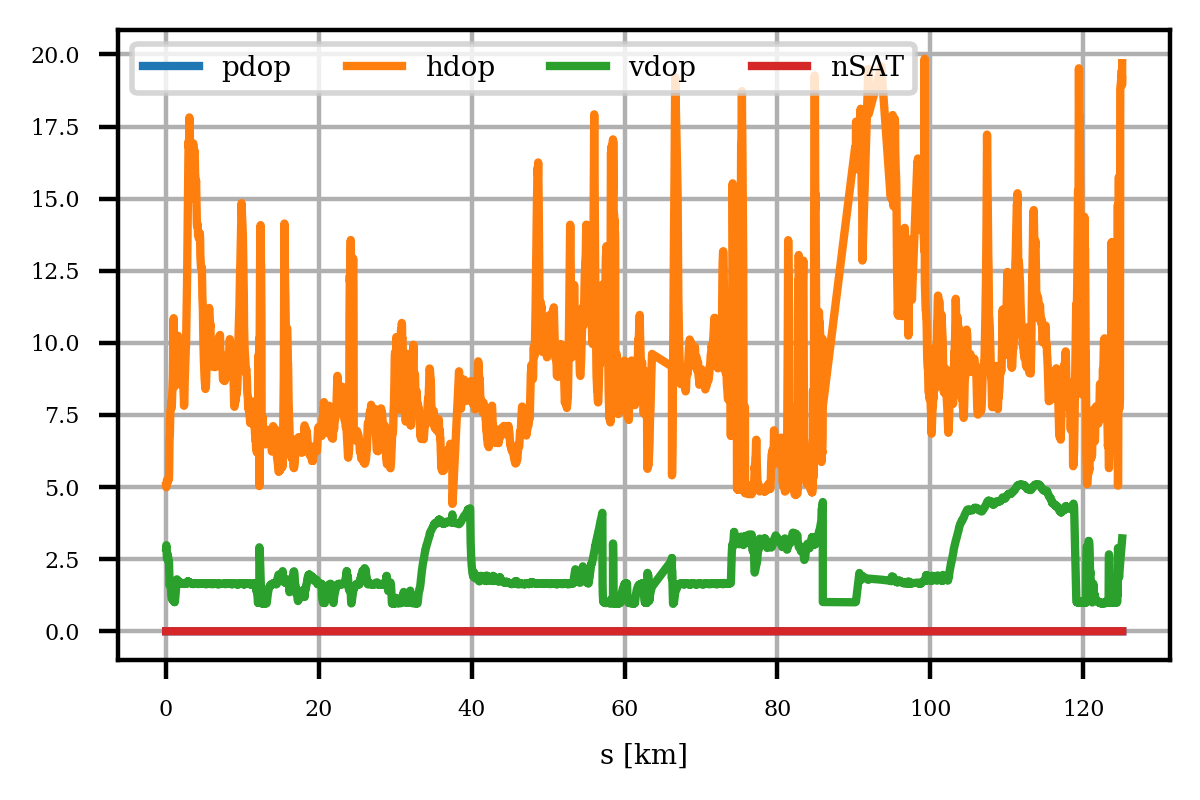
\includegraphics[width=\textwidth]{Route/cond_dop_IPhone 11 Pro.png}
		      	   \caption{Conditioned data}
		      	   \label{fig:iPhone_cond_dop}
		     	\end{subfigure}
		      \caption{iPhone 11 Pro - DOP and number of satellites - route profile}
		      \label{fig:iPhone_dop}
			\end{figure}
			\begin{figure}[h]
		    	\centering
		     	\begin{subfigure}[b]{0.45\textwidth}
		      		\centering
		      	   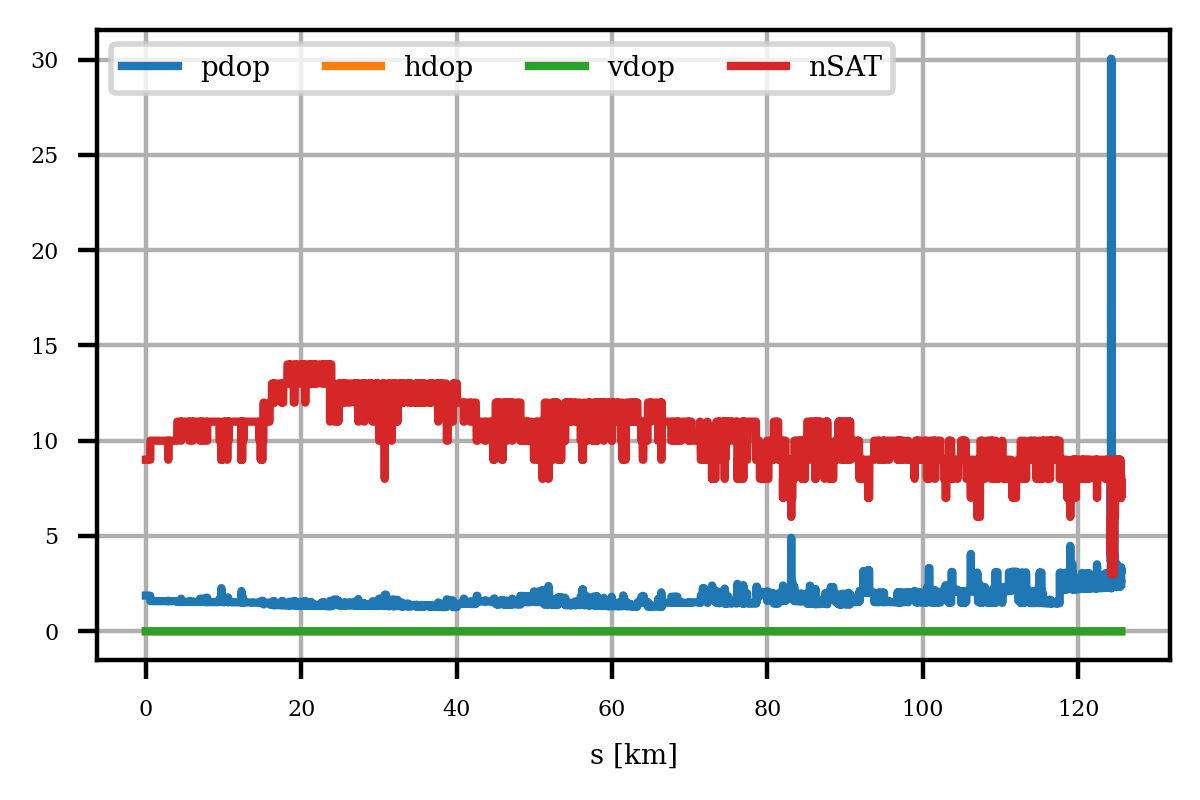
\includegraphics[width=\textwidth]{Route/raw_dop_U-blox M8N.png}
		      	   \caption{Raw data}
		      	   \label{fig:Gadget1_raw_dop}
		     	\end{subfigure}
		     	\begin{subfigure}[b]{0.45\textwidth}
		      	   \centering
		      	   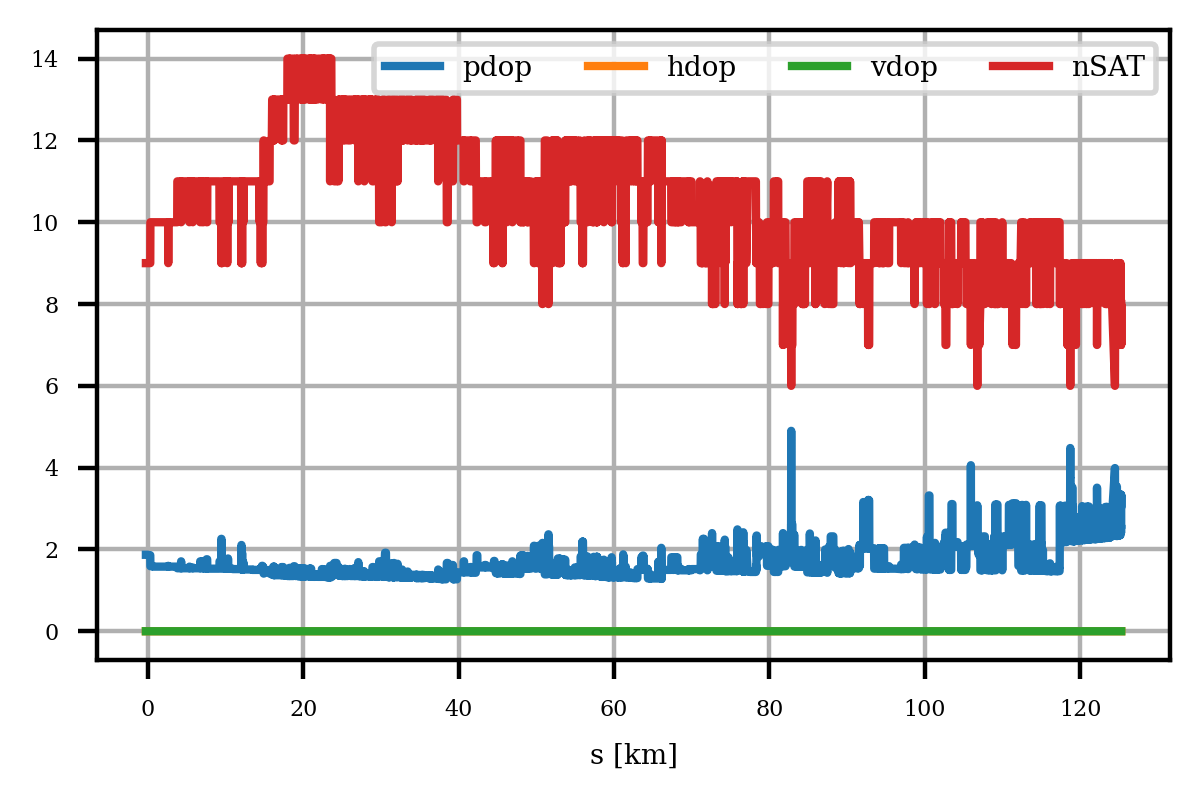
\includegraphics[width=\textwidth]{Route/cond_dop_U-blox M8N.png}
		      	   \caption{Conditioned data}
		      	   \label{fig:Gadget1_cond_dop}
		     	\end{subfigure}
		      \caption{U-blox M8N - DOP and number of satellites - route profile}
		      \label{fig:Gadget1_dop}
			\end{figure}
			In case of the iPhone the horizontal and vertical DOP values are available. Stable low values can be found in the beginning of the route staying below 2.5. This increases at the middle section of Gödöllő Hills up to 5.0 and then reduces at arriving to Budapest to around 3.0. After clearing the data we can deduct that the horizontal DOP values range between 5 and 20 and the vertical DOP values range between 1 and 5. The variance of the horizontal DOP is increasing as the train is heading for Gödöllő and Budapest. The number of satellites are not recorded by the iPhone. The results of the U-blox M8N measurement shows the number of satellites, mostly over 9 satellites considered for positioning, also the positional DOP is highlighted which shows low rates but a steady increase on the way to Budapest. After removing the outlyers the number of satellites range between 6 and 14 and the positional DOP changes between 1 and 5, mostly fluctuating around 2. This concludes a moderate to fair accuracy rating for the iPhone and an excellent rating for Gadget one based on the categorization of \cite{tahsinAnalysisDOPIts2015}.
	\section{Discussion}
		Static measurement show a positioning accuracy of 9,57 m and 16,80 m for U-blox M8N and MTK 3339. The exact definition of track tracjectory is difficult with such achived values, however for dynamic vehicle simulation the changes of the trajectory (elevation, track radius) will be in focus. Considering this and increasing the number of measurements to statistically increase the accuracy might lead to a precision level that allow the use of obtained track data. It is noteworthy that the iPhone did not record values, this makes difficult to precisely record the station positions where the train is standing still and these single points can be considered as outliers and easily removed during data processing. This was proved during the processing of the route profile as some stations were removed from the profile. \\
		The dynamic measurement proved that the route profile can be recorded with these tools, similar charateristics can be achieved after data processing. The downturn of the measurement was to realize the some receivers might adopt internal algorithm to provide data only if a certain change is happening in the calculated location parameters. This was the case for MTK 3339 where the evaluation of the dynamic measurement can not be considered due to the delayed update of the speed values. Besides that both for the iPhone and for the U-blox M8N the measured speed profile and altitude profile show good correlation. The calculated accuracy shows higher rate for U-blox M8N and more robust behaviour against noises resulting in fewer outliers. \\
		The comparison of the recorded route profiles shows in general that the U-blox M8N is providing more accurate positioning and speed information than the iPhone 11 Pro. This is confirmed by the geographical location as no differences can be seen on the U-blox M8N compared to the railway tracks than the location provided by the iPhone. Although the deviation to the exact railway track trajectory is not quantified as no information is available that would allow this, the comparison with Google Maps and the continuity of the trajectory supports this observation. \\
		On the other hand contradictory results obtained from the altitude data as the iPhone shows much more accurate values than the U-blox M8N. A deeper analysis is done on this issue because higher inaccuracy is expected on the altitude data than on the latitude and longitude position. Extracting the elevation information from central database based on the latitude and longitude positions show that the height information from a central database \cite{GPSVisualizerAssign} corresponds to the iPhone recordings. This raises the assumption that during recording the iPhone solution connects to a central database via GSM to obtain more accurate altitude information. \\ 
		The speed profile shows that the recordings of U-blox M8N were more stable allowing the detection of stations and tracking the speed profile in a more detailed way. \\
		In general the accuracy figures also proved the U-blox M8N reached higher accuracy, the horizontal values of the iPhone are ranging in the moderate to fair level according to \cite{tahsinAnalysisDOPIts2015} and the signals are influenced more in the hilly section. The performance of U-blox M8N remained stable over the whole recording session and the positional DOP value remained in the excellent ranking according to \cite{tahsinAnalysisDOPIts2015}. \\
		The algorithm used for detecting and removing the outliers were effective, the additional measures taken on filtering out high DOP values also aided to rely on data with acceptable accuracy level. In case of the iPhone more points needed to be removed which led to a loss of sections of the route. A note to be taken to the sampling frequency as well, as the iPhone was limited to 1 Hz the use of Savitzky-Golay inevitably led to loss of information on the single stops at stations and on the highest peak of the altitude. To avoid this behaviour the increase of the sampling frequency in case of the U-blox M8N proved to be successful. \\
		The reliability of the different devices show a difference. The static behaviour of the iPhone makes it hard to record standstill positions while the low fix rate of MTK 3339 prevents recording correct speed profiles. U-blox M8N provided a stable and reliable data series. Additionally MTK 3339 behaved unreliable during setup, especially when setting up the sampling frequency and communication baud rate. A workaround was found to carry out the measurements but the real root cause is not yet defined which could lead to additional unpredictable behaviour. \\
		In terms of usability and configuration the iPhone shows the least possibilities as all the configuration is predefined in the OS or in the application used, therefore further fine tuning is not easily possible. The protocol of MTK 3339 offers the basic functionality for configuration which covers the setup of the GNSS systems, communication and sampling rate, however the communication with the receiver proven to be unreliable. The protocol description of MTK 3339 is the most comprehensive and offers several options for configuration. It allows the use of it's own UBX protocol where a self-made parser is easy to be developed resulting in a more robust design of the tool.
	\section{Conclusion}
		A comparative study is conducted to assess the capabilities of different tools to record railway vehicle route profiles with the intention to use this data later to vehicle dynamic simulation. Two tools are developed and compared with each other and a mobile phone. Field recordings performed to acquire real life route profile information. The gathered data is analyzed by comparing the datasets recorded with the different tools and assessing the accuracy level based on available general GNSS information. \\
		The static measurement shows that the U-blox M8N and MTK 3339 works properly and provides position information at an acceptable level, however the iPhone's internal configuration prevents it from using. The dynamic measurement show that the iPhone and U-blox M8N is able to record route profiles while the MTK 3339 faced a speed update issue that prevented it from further use. Field recording proves that it is possible to record the route profile with iPhone and Gadget however MTK 3339 failed during setup. The comparison measurement shows that the developed U-blox M8N is able to gather more reliable satellite signal and provides more accurate position and speed information compared to the iPhone when using for recording railway vehicle routes as described in this paper. \\
		Based on the results achieved and the experience gathered in robustness, reliability and configurability the final conclusion is to use the U-blox M8N for later research purposes. However survey on the available new products and technologies should be done from time to time to update the measurement equipment in the future. \\
		It has to be noted that none of the tools were optimized for this use case, easily available hardware and software were used during the study and the required accuracy for the purpose of obtaining data for railway vehicle dynamic simulation is not defined at this stage of the research.
	\newpage
	\printbibliography
\end{document}
